\documentclass[a4paper,oneside,12pt]{book}
\usepackage[utf8]{inputenc}
\usepackage{helvet} 
\usepackage[T1]{fontenc}
\renewcommand\familydefault{\sfdefault}

\usepackage{pdfpages}
\usepackage{float}

\usepackage{NWUStyle}

\usepackage[edges]{forest}

\definecolor{foldercolor}{RGB}{124,166,198}

\tikzset{pics/folder/.style={code={%
    \node[inner sep=0pt, minimum size=#1](-foldericon){};
    \node[folder style, inner sep=0pt, minimum width=0.3*#1, minimum height=0.6*#1, above right, xshift=0.05*#1] at (-foldericon.west){};
    \node[folder style, inner sep=0pt, minimum size=#1] at (-foldericon.center){};}
    },
    pics/folder/.default={20pt},
    folder style/.style={draw=foldercolor!80!black,top color=foldercolor!40,bottom color=foldercolor}
}

\forestset{is file/.style={edge path'/.expanded={%
        ([xshift=\forestregister{folder indent}]!u.parent anchor) |- (.child anchor)},
        inner sep=1pt},
    this folder size/.style={edge path'/.expanded={%
        ([xshift=\forestregister{folder indent}]!u.parent anchor) |- (.child anchor) pic[solid]{folder=#1}}, inner ysep=0.6*#1},
    folder tree indent/.style={before computing
     xy={l=#1}},
    folder icons/.style={folder, this folder size=#1, folder tree indent=3*#1},
    folder icons/.default={10pt},
}


\tolerance=1
\emergencystretch=\maxdimen
\hyphenpenalty=10000
\hbadness=10000
%================================================================================

\begin{document}

\Title{Identifying StyleGAN images}
\Initials{N}
\FirstName{Neil}
\Surname{Foxcroft}
\StudentNumber{28418077}
\ORCID{0000-0002-8389-8826}
\MScorPhD{Bachelors Honours}
\Field{Computer Science and Information Technology}
\Supervisor{Dr. R. Serfontein}
%---------------------------------------------

\MakeTitle %This command creates the Title page.


%-------------------EDIT----------------------
%Type your acknowledgements:
\begin{Acknowledgements}{}
			I would like to thank the following persons for their support and guidance throughout this project that enabled me to complete it successfully.
			
			Dr. Rudi Serfontein, Thank you for your insight and support in my research project and always being there to answer any questions I had. Your guidance enabled me to complete the project successfully and professionally. 
			
			Prof   Tiny Du Toit, Thank you for the knowledge you shared with me regarding anything related to artificial intelligence. As a master in your craft it was helpful to learn from you. Thank you for making available your GPU that helped me train a portion of my artefact on.
			
			Manre' van Zyl, Thank you for your help and support and the collaboration in the Labs throughout the year.
			
			Affaan Muhammad, Thank you for your insights and input and the support provided throughout the year.
\end{Acknowledgements}
%---------------------------------------------


%-------------------EDIT----------------------
%Type your abstract:
\begin{Abstract}{}

The creation of a Style-Based Generator Architecture for Generative Adversarial Networks (StyleGAN) introduced the world to the possibility that images can be generated in such a way that it is difficult for a human to detect that these images are not real. A study conducted on StyleGAN and Convolutional Neural Networks helped in the identification of these images. A was created artefact that demonstrate the proposed neural network solution method. The created CNN proved that this method of detection resulted in promising results. To improve the detection accuracy further the hyperparameter optimization framework Optuna was implemented on the neural network and dataset to increase the model's accuracy drastically. Hyperparameter optimization is a powerful tool in machine learning that can structure a neural network architecture in such a way that massive gains are made in the networks predictions. To allow for easy interaction a Front-end web application formed part of the artefact  and the Flask framework was used for the model implementation and the user interface. Uploading images to the application will provide users with feedback whether or not a specific image was generated using StyleGAN or if the image is that of a real human being. 

\textbf{Keywords:} Convelutional Neural Network, Flask, Hyperparameter Optimization, Machine Learning, Neural Networks, Optuna, StyleGAN
			%Provide all of your keywords here (separated by semi-colons. This will appear below the abstract.
\end{Abstract}

\begin{Opsomming}{}


Die skepping van 'n stylgebaseerde skeppende argitektuur vir generatiewe teëstanderige netwerke (StyleGAN) het die wêreld bekendgestel aan die moontlikheid dat beelde op so 'n manier gegenereer kan word dat dit moeilik is vir 'n mens om vas te stel dat hierdie beelde nie werklik regte beelde is nie. 'n Studie wat op StyleGAN en 
Konvolusiese Neurale Netwerke gedoen is, het gehelp met die identifisering van hierdie beelde.  'n Artefak was geskep wat die voorgestelde neurale netwerk oplossing metode demonstreer. Die geskepte KNN het bewys dat hierdie metode van identifikasie belowende resultate tot gevolg gehad het. Om die identifikasie akkuraatheid verder te verbeter, is die hiperparameter optimeringsraamwerk Optuna op die neurale netwerk en datastel geïmplementeer om die model se akkuraatheid drasties te verhoog. Hiperparameter-optimering is 'n kragtige instrument in masjienleer wat 'n neurale netwerkargitektuur op so 'n manier kan struktureer dat massiewe winste gemaak word in die netwerkvoorspellings. Om maklike interaksie moontlik te maak was daar 'n webtoepassing deel van die artefak ontwikkel en die Flask-raamwerk is gebruik vir die modelimplementering en die gebruikerskoppelvlak. Die oplaai van beelde na die toepassing sal gebruikers terugvoer gee of 'n spesifieke beeld met StyleGAN gegenereer is en as die beeld dié van 'n regte mens is.

\textbf{Sleutelwoorde:}  Flask, Hiperparameter-optimering, Konvolusiese Neurale Netwerk, Masjienleer, Neurale Netwerke, Optuna, StyleGAN

\end{Opsomming}
%---------------------------------------------


\MakeTOCandLOFandLOT %This command creates the table of contents, list of figures and list of tables.


%-------------------EDIT----------------------
%[OPTIONAL] Type your table of abbreviations. Delete this if you do not intend to use it.
\begin{TableOfAbbrev}
			A table containing a list of abbreviations in the order of appearance, that will be used throughout text.
			\begin{table}[!htpb!]%
			\begin{tabular}{ll}
			\textbf{StyleGAN} & a Style-Based Generator Architecture for Generative Adversarial Networks\\
			\textbf{GAN} & Generative Adversarial Network\\
			\textbf{AI} & Artificial Intelligence\\
			\textbf{DSRM} & Design Science Research Methodology\\
			\textbf{SWOT} & Strengths, Weaknesses, Opportunities and Threats\\
			\textbf{PaaS} & Platform as a Service\\
			\textbf{IaaS} & Infrastructure as a Service\\
			\textbf{VS Code} & Visual Studio Code\\
			\textbf{px} & pixles\\
			\textbf{URL} & Uniform Resource Locator\\
			\end{tabular}
			\end{table}
\end{TableOfAbbrev}

\pagestyle{fancy}
\setcounter{page}{1}
\fancyhead{}
\renewcommand{\headrulewidth}{0pt}
\fancyfoot[c]{\thepage}
\pagenumbering{arabic}

\chapter{Introduction}\label{ch1}

The creation of a Style-Based Generator Architecture for Generative Adversarial Networks (StyleGAN) and similar technologies introduced the world to the possibility that images can be generated in such a way that it is difficult for a human to detect that these images are not real and instead generated by a neural network. With this proposed research project, the StyleGAN technology will be thoroughly studied to determine how an approach can be developed to identify artificially generated images to enable the detection of these falsified identities that used the StyleGAN technology. An artefact will demonstrate the proposed solution methods function and convey the successful method in a practical environment with the use of StyleGAN generated images and images retrieved from the Flickr Faces dataset to evaluate the method. The following section is the proposal for the research project and will form the first chapter of this proposed project.



% \begin{figure}[!htbp!]%
% \centering
% 
\includegraphics[width=0.4\textwidth]{img/NWU}%
% \caption{The first figure. The old university logo and colours.}%
% \label{fig:1}%
% \end{figure}

% \begin{figure}[!htbp!]%
% \centering
% \includegraphics[width=0.4\textwidth]{img/NWU2}%
% \caption{The second figure. The new university logo and colours.}%
% \label{fig:2}%
% \end{figure}


\section{Project Description}

StyleGAN is an open-source Generative Adversarial Network (GAN) that can be used to generate faces of people that do not exist (such as those shown on \href{https://www.thispersondoesnotexist.com}{thispersondoesnotexist.com}). This means that fraudsters can use StyleGAN generated faces that normally would pass a visual inspection conducted by a human inspector as part of false identities. The detection of such images with the use of artificial intelligence will be useful because of the factors that currently lead to misidentification.

\section{Project Background}

In this modern world with humanity currently in its 4th industrial revolution, the additions of innovative technologies require original approaches to implement and maintain these technologies. The change from the digital age to the automation age is accelerated by breakthroughs in the fields of Artificial Intelligence (AI) and security \citep{Skilton2017}.

One of the big advances in AI is the creation of StyleGAN, this new approach to a GAN allowed for more control in an image than its predecessors \citep{Karras2019}. StyleGAN uses the principles of a GAN to create new images derived from input that specifies what “styles” need to be included in the image. According to \cite{Karras2019} a style is defined in this context as a set of parameters that modifies the input of the image to result in different outputs. If the input received is that the image needs to be in the style of a person with glasses, red hair and must be female, StyleGAN will then generate that image based on images used of that similar styles in the initial training of the model. The resulting image will thus be that of the “styles” required in the input. While this functionality can be utilized for various positive use cases – this breakthrough also creates various challenges and setbacks in the field of security, more specifically the aspects of facial recognition and identity verification as malicious use of this GAN might aid in the creation of fraudulent identities \citep{Mitra2021}. Figure \ref{fig:1} demonstrates how an image can be altered with the use of StyleGAN by specifying what style changes should be made on that image.

The styles applied in figure \ref{fig:1} demonstrate the capabilities of StyleGAN and further illustrate the possible difficulties of detecting that these images were generated with a GAN \citep{Karras2019}. Possible misidentification of StyleGAN images is a reality that needs to be addressed. Humans in the role of identifying artificially generated human faces may be susceptible to external factors hindering their capabilities and increasing the rate of error in which they identify fraudulent images \citep{Fysh2018}. \cite{Fysh2018} also noted that in the specific use case of passport officers that were tested on passport images captured on the same day against the “traveller” presenting that image, that the officers made substantial errors in a controlled environment when comparing the picture identity to that of the traveller. These results enforced their original statement that humans struggle with unfamiliar face identification.

\begin{figure}[H]%
\centering
\fbox{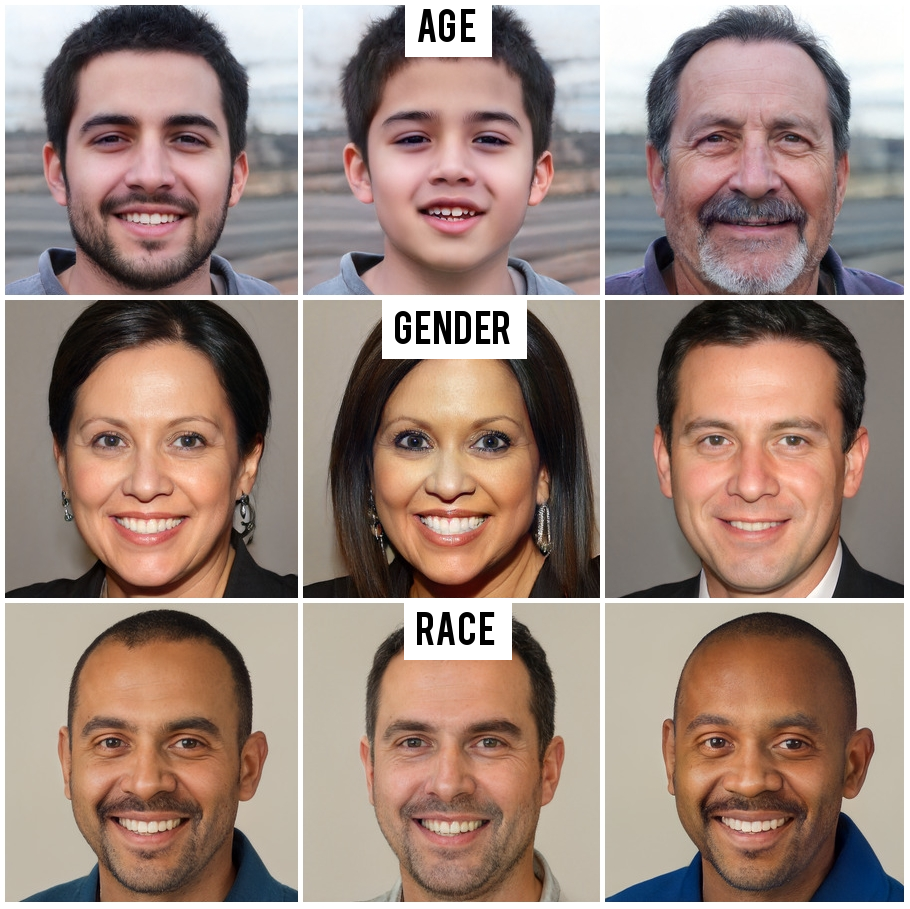
\includegraphics[width=0.8\textwidth]{img/f1.png}}%
\caption{Applied "styles" on images using StyleGAN that demonstrates styles and the resulting changes adapted from \cite{Karras2019}}%
\label{fig:1}%
\end{figure}

Opportunities for fraud escalated with the recent boom in online applications. This bigger threat for fraud is exaggerated in the mobile market due to the high volume and demographic variety of current mobile users \citep{Mitra2021}. Most applications require user accounts and the unique user’s identity is commonly the specific value the application requires. Examples of this in practice is online dating applications namely Bumble, Tinder and Hinge. These free to use applications allow multiple users to connect and interact where interaction mostly starts because of the user’s interaction with the images displayed on a profile. This emphasis on the gallery of a user profile creates a unique opportunity where StyleGAN can help cyber criminals fake identities within these apps. Fraudulent use of StyleGAN in this environment can directly lead to an increase in catfishing incidents. Catfishing is the act of deceiving an individual with the use of a specific fictional identity and persona to gain assets that are usually in the form of financial gains or personal information \citep{Chandler2016}. These apps usually have various systems in place to combat such fraudulent actions by requiring account verification. The verification process requests that a user submit one or multiple images where they pose in specific ways. StyleGAN can successfully counter these forms of verification as an image can be generated wherein a person perform specific poses \citep{Karras2019}.

Because of StyleGAN’s ease of use and availability more fraudsters used it to create false accounts on popular social media platforms since its creation. Facebook took down an undisclosed number of accounts in December 2019 that had reportedly made use of StyleGAN to generate realistic profile pictures for establishing false identities on their site \citep{Gallagher2019}. This emphasized the possible threat StyleGAN poses to the security of individuals and the IT industry. Because of the threat, StyleGAN poses the need for a method to detect these generated images is identified.

StyleGAN was released to the public in December 2018 with all its packages and source code. This novel approach to GAN’s that was developed by Nvidia demonstrated its possible capabilities by the accompanying portraits of convincing human faces. The big leap forward in this technology was the realism brought to the GAN’s generated faces dataset that is close to real human beings and not easily detected by humans \citep{Fleishman2019, Karras2019}.

StyleGAN was popularised because of a former engineer at Uber, Phillip Wang’s website \href{https://www.thispersondoesnotexist.com}{thispersondoesnotexist.com} that was released in February 2019. Phillip’s main goal when publishing this website was to educate the public on how GAN’s work and the dangers that they might pose to the average user. Phillip achieved this by specifically emphasizing StyleGAN and its realistic human face generation capabilities \cite{Fleishman2019}. The goal of making more people aware of StyleGAN and possible fake identities was also promoted by another website. Two members of the University of Washington created the website \href{https://www.whichfaceisreal.com}{whichfaceisreal.com} \cite{Fleishman2019}. This website allows users to select an image between a StyleGAN image and a verified human image. This online tool helped users realise that the differences between computer-generated images and real images are only decreasing with the advancement of technology.

The big advancement in StyleGAN that increased the need for this proposed project was the release of StyleGAN2 in February 2020 \citep{Karras2020}. Following the release of version 2, there were improvements in the generation process of these images with this updated version of StyleGAN. StyleGAN2 saw that images were no longer subverted with artefacts or traces left on the image because of the processing method used in the previous iterations \citep{Karras2020}. These traces were easy to identify and clearly showed out of place in the context of the image. With the removal of the traces, usually, in the form of drop-like spots, the difficulty in detecting the generated images increased and similarly the need to detect StyleGAN generated images used maliciously in security verification processes.

By looking at how the technology has been used since its release, the possible use-cases for GAN generated images and the always growing cybercrime industry the possible detection of these images is identified as a crucial function in the 4th industrial revolution. With these identified factors will the proposed project aim to solve the problem of detecting StyleGAN images by using an artificial intelligence approach to solve the problem.

\section{Research Question}

With the identified need for detection of StyleGAN images and the discussed security implications that the invention of StyleGAN and similar methods introduced the proposed project aims to detect these images with the use of a trained neural network. The main research question that this proposed project aims to answer is: How can StyleGAN generated images be detected?

\section{Aims and Objectives}
\subsection{Aims}

The main purpose of the proposed project is to develop a method that can detect fraudulent human faces created by StyleGAN with relative accuracy. Various techniques and approaches to the detection of GAN generated images will be researched and the simplest implemented approach that can still detect these types of images with relative surety will be selected for the artefact.

\subsection{Objectives}

The success of the project will be weighed against the completion of the secondary objectives that have been identified as listed below.

\begin{itemize}
	\item Perform a literature study on GAN's and specifically analyse the architecture and function of StyleGAN to understand the technology.
	\item Develop an approach to the successful identification of generated images.
	\item Develop an artefact that will use the selected method to detect a fake identity. 
\end{itemize}

The successful completion of the above-identified objectives will aid the researcher in satisfying the aim of the proposed research project.

\section{Procedures and Methods}

This section will describe the research paradigm and the methodologies that will be used to complete the proposed project. By examining the chosen paradigm, methodology and artefact life cycle in an academic viewpoint with specific reference to information systems design and development will the most applicable approaches in these sections be identified and selected. The data that will be captured in the development phase and reviewed in the testing phase will be discussed.

\subsection{Paradigm}

Positivism is a research paradigm that is focused on the world view that “factually accurate” knowledge is gained through the observations made by the observer. In positivistic studies, the research is confined to only the collection of data and the interpretation of this data to gain knowledge and insight into the problem. Positivism requires the researcher to only make quantifiable observations that can directly lead to statistical analysis. With the use of this paradigm, the researcher must reject intuitive knowledge because it cannot be justified by sensory experiences and is thus subjective to the researchers own interpersonal influences. Positivism as a philosophy is justifiable by empiricist views that knowledge stems from a human experience \citep{Collins2018}.

The positivistic research paradigm is suitable for the proposed project because with the creation of the artefact, the data collected will be examined and an unobjective interpretation of the data is necessary. The data collected will be the results of the artefact’s successful identification of StyleGAN generated images. 

\subsection{Methodologies}

Methodologies determine the structure of completion for a specific project. With this proposed project the researcher will study the technology that enables StyleGAN to generate images. To aid in the research process and the development of the artefact the Design Science research methodology (DSRM) will be used throughout the proposed project \citep{Peffers2007}.

DSRM is an information systems specific methodology that focuses on research and iterative design \citep{Peffers2007}. Because the researcher is studying the field and technologies in which they want to solve the specific problem the background knowledge of the problem will be explored parallel to the design of the problem solution. DSRM will enable iterative design and development throughout the completion of the proposed project.

\subsection{Artefact Life Cycle}

With the use of the DSRM, the researcher will amend the project with the acquisition of new knowledge. The artefact will be developed while research is conducted on the technologies required, thus the artefact development will similarly be conducted in increments. The implementation of the Agile methodology for the development of the artefact will be suitable as Agile accommodates changes in artefact scope, planning and incremental deployments of preliminary artefacts \citep{Weiyin2011}.

The artefact that will be developed will aim to detect StyleGAN generated images between a data set of real images of human faces and StyleGAN generated images. The artefact can be hosted online if needed as this increase its compatibility and deployment reach across multiple platforms. Because of these factors, Agile will be the most suitable methodology for artefact development. 

\subsection{Data Capture}

The data captured in this project will be collected and displayed to the user in the web application to aid in the demonstration of the artefact, and method of detections success in the finalization phase of the project. Data that will be captured is the number of images used in the training of the models, the number of images that were used throughout the identification testing phase and the accuracy of the chosen identification method. These statistics will help the researcher determine the success of the chosen method of detection.

\section{Project Management and Project Plan}

\subsection{Scope}
The research of the technologies implemented in StyleGAN and the specific architecture of StyleGAN is important for the design of a suitable approach for the detection of these images. The scope of this research is the identification of images, the use of artificially generated human faces, security concerns when determining identities based on profile images and the research of neural network's that will be a possible technology used for the solution to the problem.

Because of the time of StyleGAN3 and 2 individual releases and the initialization of the proposed project the scope of this project will only focus on the detection of StyleGAN1 generated images. 


\subsection{Limitations}

Possible limitations that can be faced during the proposed project will hold back advancements that the researcher aims to complete in this study. The limitations thus need to be identified and addressed to ensure the completion of the proposed project within the specified period. The proposed project will make use of neural network's and image processing technologies to answer the research question. These technologies require large computing capabilities for the training of neural network models. This will be addressed by using cloud services instead of traditional hardware. Cloud services provide a more cost-effective approach to large computing needs.

\subsection{Risks}

Possible risks that can be identified that this proposed project is susceptible to include the risk that the scope of the project is not adhered to. The scope defines the boundaries in which this proposed project will take place, therefore careful adherence to the scope will ensure that the research is relevant to the initial project that was proposed. The responsibility of staying within the scope of the project lies in the researcher proposing this project.

\subsection{Strengths, Weaknesses, Opportunities and Threats}

The Strengths, Weaknesses, Opportunities and Threats (SWOT) of this proposed project can be evaluated using a SWOT-analysis table. The risks and limitations mentioned previously is also mentioned when conducting a SWOT analysis. Figure \ref{fig:2} shows the SWOT analysis of the proposed project.

\begin{figure}[H]%
\centering
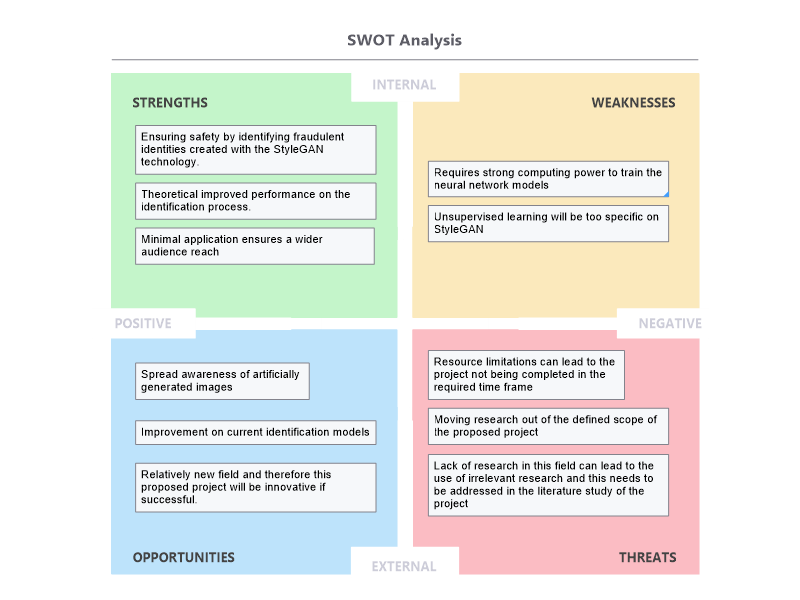
\includegraphics[width=1\textwidth]{img/SWOT.png}
\caption{SWOT analysis in the Identification of StyleGAN images}%
\label{fig:2}%
\end{figure}

\subsection{Timetable}

The proposed project will start on the 16\textsuperscript{th} of February 2021 and will be finalized and completed on the 8\textsuperscript{th} of November 2021. This project will be subdivided into 3 phases each with separate deadlines. The first phase is the research proposal that will be concluded on the 18\textsuperscript{th} of April 2021. The second phase involves research that will require an in-depth analysis of the problem, possible solutions, and the discussion of StyleGAN in a literature study that must be completed on the 13\textsuperscript{th} of June 2021. The last phase is the development of an artefact to practically demonstrate the solution to the identified problem. Phase 3 of the proposed project will also require a demonstration of the developed artefact and a video demonstration of the project on the 1\textsuperscript{st} of November 2021. The submission of the whole project must be completed and the final documentation will take place on the 8\textsuperscript{th} of November 2021. The Gantt chart in figure \ref{fig:3} graphically displays the preliminary project planning with the tasks in the required sequential order for the successful completion of the proposed project. The adherence to the project planning and the preliminary Gantt chart will enable the researcher to effectively divide the tasks into manageable time frames. The prerequisite tasks are required to begin with a dependent task and are displayed graphically in figure \ref{fig:3}.

\begin{figure}[H]%
\centering
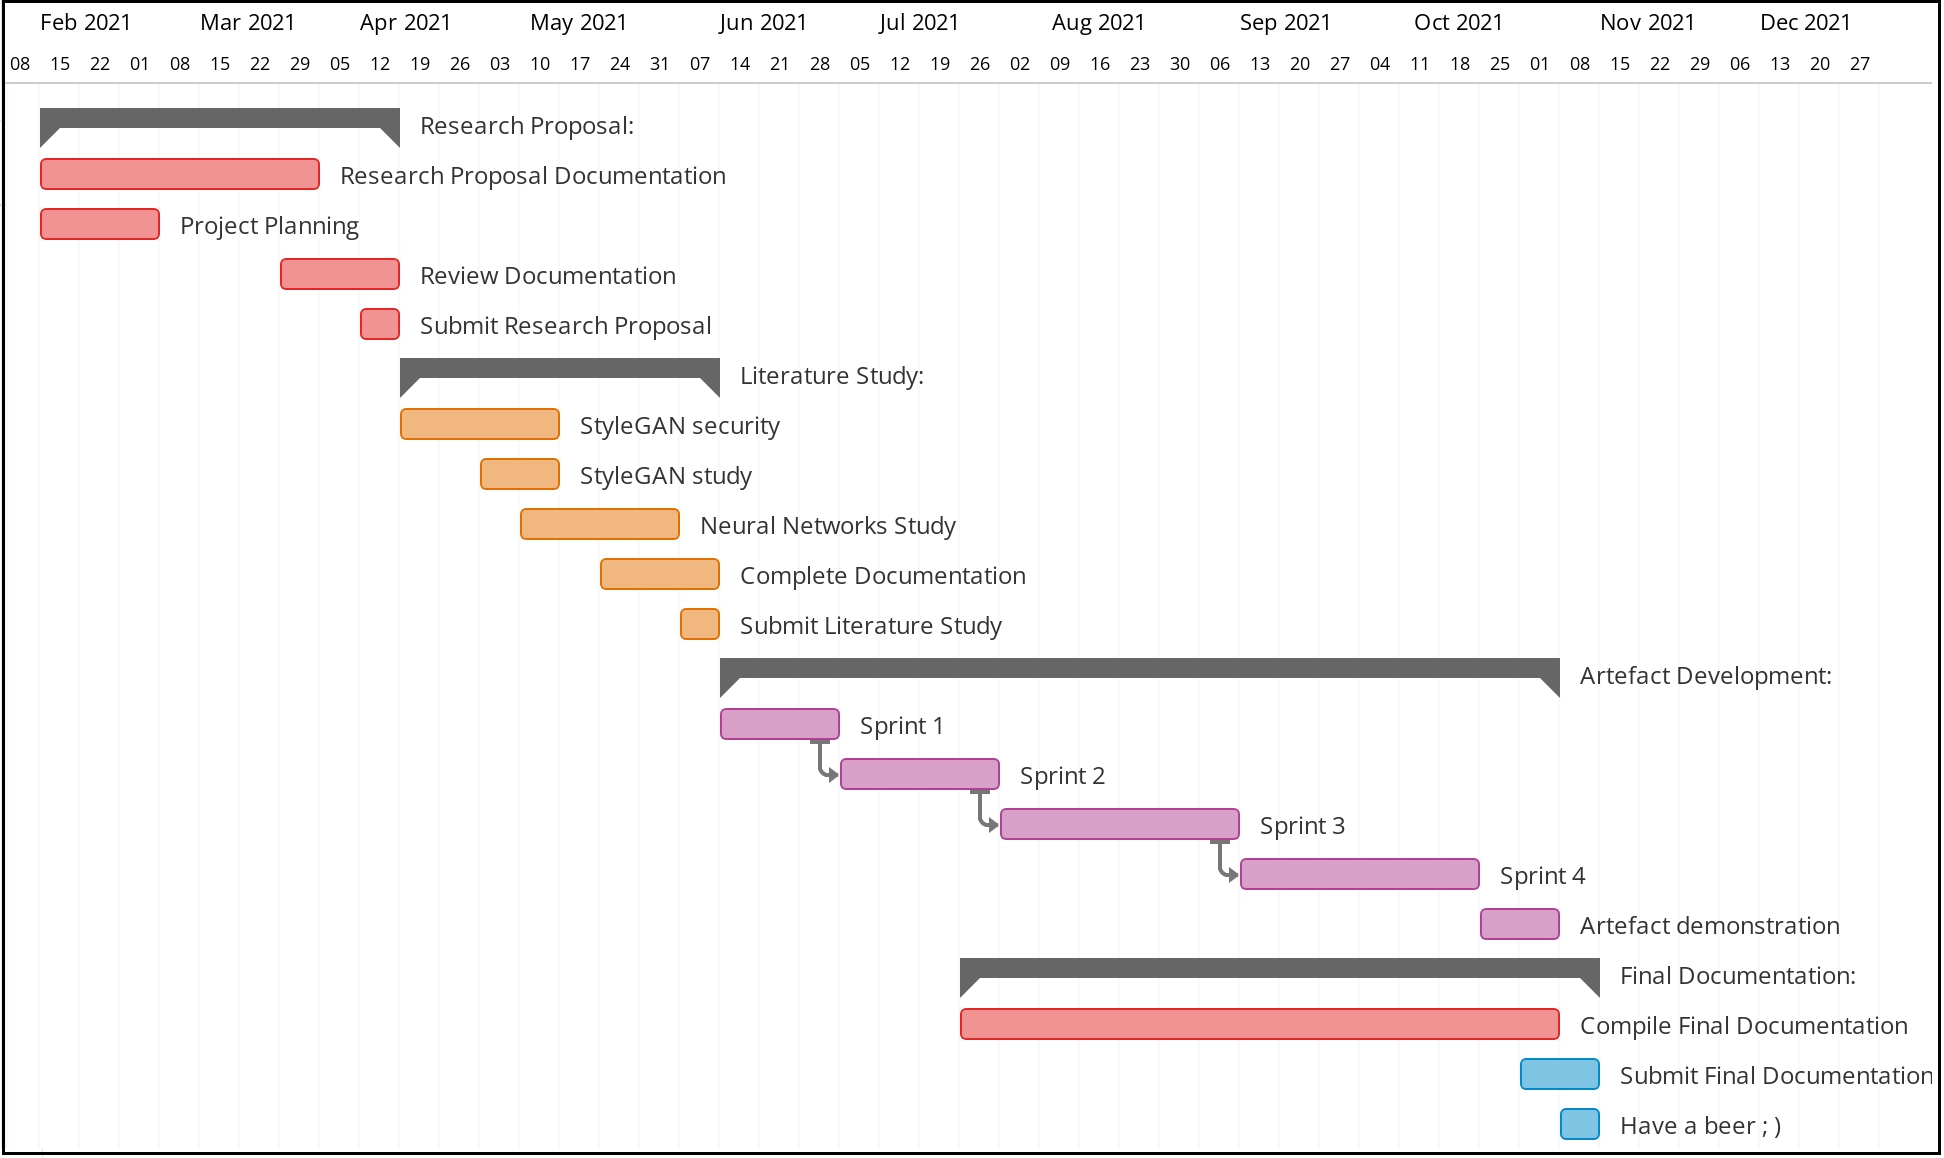
\includegraphics[width=1\textwidth]{img/ganttfinal.png}%
\caption{Gantt Chart graphically demonstrating the planned schedule of the proposed project}%
\label{fig:3}%
\end{figure}

In figure \ref{fig:3} time management and planning is clearly shown to be crucial for the completion of the proposed project. The artefact development planning is subject to change based on the research outcomes and findings of the researcher in this proposed project. 

\section{Development Platform, Resources and Environment}

The development of the artefact will be conducted in parallel with the research on the subject. Development of the GUI will be conducted at the same time as the literature study. The development of the final artefact and method of detection will only be conducted after the literature study based on the knowledge acquired in that phase. With the knowledge gained in the literature study will the specific method to detect StyleGAN images be implemented into the artefact. The artefact development platforms, resources and environments will be discussed in this section.

\subsection{Web Application}

The artefact will be a web application that can be scaled and hosted through a cloud services provider. The language that will be used for the front-end web application is Python-based using the scaled-down Django framework, Flask. For the implementation of the method for detection of StyleGAN generated images the language used in the back end of the artefact will be Python. The reasoning behind the selection of the above-mentioned technologies is discussed in the following section.

Developing a web-based application allows for further reach and compatibility compared to historical installation software \citep{murugesan2011}. Developing a simple web application with a minimalistic front end will users more intuitively be able to use the application and will improve complex implementations ease of use \citep{murugesan2011}. Web apps opened in the browser natively scale to be available on various devices and screen sizes. For the StyleGAN artefact, improved availability will provide the application with a wider reach and therefore more artificially generated images can be detected. 

The web application will allow a user to load a new image where the artefact will then classify that image as a StyleGAN generated image or a real human image. The web application must keep track of basic statistics and provide them to the user. The basic statistics that will be provided in the artefact of this proposed project will be the neural network's confidence in its prediction. An uncomplicated design will be implemented where the user can intuitively navigate the web page.

\subsection{Python}

For the backend of the proposed project Python will be used. Python is an intuitive programming language that due to its active community has an abundant set of resources available to use in the artificial intelligence field. Python is widely used for artificial intelligence applications and thus is a suitable programming language to code the chosen method of detection.

\subsection{Flask}

For the front-end of the artefact’s web application Flask will be used. Flask is a framework based on the larger framework Django that is a web framework using the Python language. Flask front-end features can use CSS-styling and the use of bootstrap will make the front-end uniform that enables faster development without the need for extensive visual design. Flask will enable the artefact to be used on multiple devices with a lightweight package without the explicit code and design to accommodate those devices. The framework natively scales assets to fit a wide range of devices.

\subsection{Jupyter Notebook}

Jupyter Notebooks is a Docker-like implementation of python coding. In a Jupyter notebook cells can be run individually allowing for more control when developing neural network's. Most cloud services use Jupyter notebooks when implementing python code on their platforms.

\subsection{Cloud Services}

Because of the possible processing resource requirements that the detection of StyleGAN images require, the training of the neural network model will be conducted on the platform and infrastructure that is provided by Google Colab.

\subsubsection{PaaS and IaaS}

In cloud services, there are multiple forms in which the cloud can be implemented for use by an individual or organisation. These implementations can range from Software to Infrastructure offered to the entity from the cloud services provider \citep{pfleeger2002}. For this proposed project there is a need for a platform and infrastructure as the training using large image datasets require processing power. Platform as a Service (PaaS) is a service model where the client develops software by using the languages and tools offered by the cloud services provider \citep{pfleeger2002}. Infrastructure as a Service (IaaS) is the second service model this proposed project will require. In IaaS the cloud services provider offers the use of processing resources and storage to name a few, to the client \citep{pfleeger2002}. A combination of IaaS and PaaS will be required for the completion of the artefact in this proposed project. 

\subsubsection{Google Colab}

Google Colab is a free-service that Google offers to data scientist to use for the development of neural network's. Google Colab workbooks is the development platform in which programming is conducted that is similar to Jupyter Notebook development on local machines. The difference in using Google Colab is the increased system resources of the web based virtual machine. Using Google Colab for the development in this project will have the benefit of the GPU attached development environment where a Nvidea K80 GPU with 12GB of RAM can be used.

\subsubsection{Google Drive}

Google Drive is a storage solution offered by Google that is integrated in Google Colab. The large datasets can be uploaded to a NWU google accounts drive, where storage is unlimited. The dataset can be mounted in Google Colab using Google Drive.

\subsection{Visual Studio Code}

Visual Studio Code (VS Code) will be the selected IDE for the development of the artefact. VS Code allows for extensions that enable easier programming practices. ESLint is an automated code formatting and standardizing tool that was developed by Nicholas C. Zakas in June 2013. With the use of ESLint all code will be the same structure and allow for easier review of code. VS Code built-in terminal is a powerful addition to the IDE and will allow for Git statements to be run in the development environment.

\subsection{Git}

For version control and deployment, the Git language will be used and the repository for the development of the artefact will be hosted on GitHub. GitHub is integrated with various cloud services and this allows the developer to easily deploy and evaluate the code.

\section{Ethical and Legal Implications}

With the development of this artefact, certain resources will be used to train the neural network. The training requires images that were generated by StyleGAN. For the comparison in the artefact images of real humans will be used.

The StyleGAN generated images are available on the official StyleGAN GitHub repository. Included in this repository is trained StyleGAN models and multiple datasets of StyleGAN generated images. The licencing of these images is stated on the GitHub repository and is a Creative Commons license by NVIDIA Corporation \citep{Karras2019}.

For the verified human faces, the preliminary dataset that will be used is the Flickr Faces dataset that was initially used to benchmark StyleGAN. The individual images were published in Flickr by their respective authors under either Creative Commons, Public Domain. All of these licenses allow free use, redistribution, and adaptation for non-commercial purposes \citep{Karras2019}.

\section{Provisional Chapter Division}

For this whole project, the following flow of the final document can be expected. These chapters will logically flow to aid in the understanding of the topic at hand and to ultimately ensure a successful artefact.

\subsubsection*{Chapter 1: Introduction}
This chapter will be concluded in the project proposal phase. It will include the research question, the project description and background. It will include the proposed project plan for the entire project.

\subsubsection*{Chapter 2: Literature Study}
This chapter will be comprised of all the necessary research to understand the project and fulfil the project aims and objectives. Mostly in this project will be focusing on the specific workings of StyleGAN to effectively detect fake images.

\begin{enumerate}
    \item StyleGAN: The history of StyleGAN and direct technologies that lead to this breakthrough in the field of GAN’s will be provided as well as the specific architecture of StyleGAN.
    \item Neural Network: This project will make use of Machine Learning and neural network's to detect StyleGAN generated images. A study will be completed on the field of artificial intelligence and how neural network's can aid in the detection of images.
    \item Hyperparameter Optimization will prove useful in improving the created neural network model to increase the detection accuracy for StyleGAN images. A Study on hyperparameter optimization methods will aid in the creation of a hyperparameter artefact.
\end{enumerate}

The study of these three sub-topics will provide the relevant background and base knowledge to develop a successful artefact and will provide the relevant foundation to improve and expand on this project in the future.

\subsubsection*{Chapter 3: Development of the artefact}

Chapter 3 will apply the chosen methodologies that were identified and discussed in Chapter 1 to enable the successful development of the proposed project's artefact. This chapter will document the artefact development phase including unfamiliar problems that are identified within the development stage. The success of the artefact will be compared to the Aims and Objectives of Chapter 1 and if they are met.

\subsubsection*{Chapter 4: Results}

The results of the Artefact will be introduced in this Chapter and the successful identification of StyleGAN images will be determined. The testing in this Chapter will identify the success of the artefact with the comparison in Chapter 4.

\subsubsection*{Chapter 5: Reflection}

Chapter 5 will summarize the entire proposed project and conclude if the problem was solved with the successful completion of the objectives of the proposed project that allowed it to fulfil the aim of the project. The limitations that impeded the proposed project will be discussed in this section. The future expansion of the project will be discussed and explained in the context of the limitations faced.

\section{Summary}




\chapter{Literature Study}\label{ch2}

The aim of this proposed project is to develop a method to detect images created by a style-based generator architecture for generative adversarial networks in a set of artificial images (generated images of human faces contained in the StyleGAN dataset) and authentic images (Flickr-Faces-HQ dataset of human faces used as a benchmark for StyleGAN). Before the aim of the project can be satisfied, a literature study is required on neural networks and StyleGAN. The basic structure of neural networks and the different types of neural networks will be researched and discussed in context with the StyleGAN technology, and the detection of StyleGAN generated images. Current detection methods will be investigated and examined to evaluate their workings and relevancy towards a StyleGAN application. In conclusion, all knowledge acquired from the literature study will be used when creating the artefact to detect StyleGAN generated images.

\section{Neural Networks}

In recent times, neural networks have been regarded as a fast-growing field offering powerful tools for most types of problem-solving \citep{Albawi}. The increased use results from the neural network's capabilities to function even with large data sets as input effectively. Therefore, a study into neural networks is required as it is a tool to use in the detection of StyleGAN generated images because of the large datasets accompanying StyleGAN. 

\subsection{History of Neural Networks}

Artificial intelligence is a modern growing field within information technology rooted in historical discoveries leading to new advances. Artificial intelligence has been in the development stages since the mid-20th century. However, early on, most advances made in artificial intelligence were developed in mathematics and computational model theory \citep{Mueller1995}.

Warren McCulloch and Walter Pitts initialised the now big field of artificial intelligence when they proposed a new general theory in information processing that artificial neurons can mimic the neurons present in the human brain \citep{Mueller1995}. \cite{Mueller1995} also notes that the neurons Warren McCulloch and Walter Pitts proposed were more simplified than biological neurons and still promised reliable computational power. The artificial neuron that could be implemented in a network to mimic a single neuron cell in the human brain and mimic the whole brain as a network is the foundation of early artificial intelligence and machine learning theory.

The next significant advance in this field came in the 1960s by researchers Caianiello and Rosenblatt. This advance resulted from focusing on two aspects of Artificial Neural Network's (ANN): 1\textsuperscript{st} being the aim to mimic their biological counterparts in their design and the 2\textsuperscript{nd} is that different structures proposed different advantages \citep{Mueller1995}. This difference of structure leading to a difference of perception is present in nature, where mammals all possess a biological brain, but the shape and network design allow mammals to think differently based on their specific computational needs\citep{Mueller1995}. Rosenblatt coined the differing structure of ANN's as the perceptron of the network, and in modern artificial intelligence theory, the perceptron is called the perception of the neural network.

The historical, theoretical initialization of neural networks is the foundation of modern neural networks. Modern neural networks' development focuses on practical applications in modern times. Neural networks are still relatively new in artificial intelligence, with theory founded in historical mathematics

\subsection{The Function of Neural Networks}

Neural networks are present in most forms of biological computation. For example, the human brain is a neural network of neurons that allow us to compute our daily tasks. An ANN mimics the human brain in its structure \citep{Krenker2011}. Like a human brain thinking through the impulses sent and received between biological neurons, an ANN sends and receives input and output through the artificial neurons in the network \citep{Krenker2011}. The neurons that form the network allow neural networks to imitate a biological brain's basic structure and computation. 

An artificial neuron is a single node within a neural network. This neuron is an independent node residing in a neural network that receives data and applies the neuron's mathematical model to this input. The output is the result of a calculation and the operation of activation and deactivation of the node.

\cite{Krenker2011} states that the neuron structure consists of three separate stages. The first stage applies the weight to the input with multiplication. The second stage is a sum function of all the previous stage weights and biases applied to the initial input. The final stage of the artificial neuron determines if the neuron should be activated or deactivated \citep{Krenker2011}. Artificial neurons activated or deactivated artificially enable the neural network to "think" and adaptively apply its computation on inputs.

\begin{figure}[H]%
\centering
\fbox{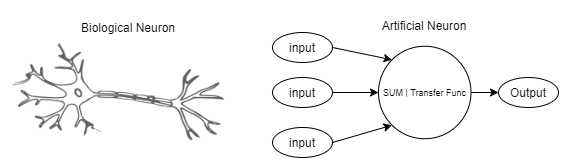
\includegraphics[width=0.95\textwidth]{img/f4.png}}%
\caption{Biological Neuron and Artificial Neuron \cite{Krenker2011}}%
\label{fig:4}%
\end{figure}

Figure 2 shows the similarities between the biological neural network and the ANN. The basis of biological neural network for the design foundation of an ANN is 

The set of neurons functioning together to form a network is called a neural network. In a biological brain, the whole cellular neurons connected in the brain and artificial intelligence are the ANN with the artificial neurons working together. ANN's are capable of processing information of real-world problems that requires a more complex approach because they can distribute their neurons in a non-linear, parallel structure \citep{Krenker2011}. Multiple neurons simultaneously are the neural network structure, and neurons do not have to flow their output into the next.

Figure 3 illustrates a primary ANN with connected neurons that mimics the structure of connected biological neurons connected inside the human brain. Each neuron within the structure of the ANN in Figure 3 can be compared to a human single brain cell in the biological brain structure. The artificial neuron present in the network only apply basic computational calculation on the data, and as output, the node only activated or deactivated itself.

\subsection{Neural Network Learning Paradigms}

Neural networks can learn in different ways, and these differences pose their respective advantages and disadvantages—the manner of learning in a neural network the network's learning paradigm.  The three different learning paradigms for neural networks used in the training of neural networks are supervised learning, unsupervised learning, and reinforcement learning \citep{Krenker2011}. The learning paradigms for neural networks are also specific to the type of data the network use in training. Concerning image classification and computer vision, only two of the three learning paradigms apply, namely supervised learning and unsupervised learning \citep{OShea2015}. Different neural network topologies use different learning paradigms. The specific choice of learning paradigm is essential in the implementation of the detection method of StyleGAN images. 

\subsubsection{Supervised Learning}

The supervised learning paradigm sets the parameters of the neural network based on the training data set it receives. The critical difference in supervised learning is that the input data is labelled before training the neural network \citep{Krenker2011, OShea2015}. The already labelled input is then compared to the output of the neural network to determine its error and accuracy. Training is applied to the network based on comparing the output the network created against the labelled input. If this paradigm is applied to the StyleGAN image detection problem, the training set of data consist of a set of images of human faces and a set of StyleGAN generated images. This input training set requires parameters or labels that identify a single image as either a human face or a StyleGAN generated image. The prediction made by the neural network will then be validated against these know classifiers on the images, and training will take place based on how the neural network predictions compare to the valid identifiers. In deep neural networks, supervised learning also deals explicitly with the labelled data. The advantages of supervised learning applied in deep neural networks such as CNN and GAN are that training can be conducted without initial knowledge about the differences between two different data inputs. The fallback to this advantageous method is that when there is outlying data present within the dataset, An image of a dog in the set of authentic images, the training can overstrain the boundary of decision \citep{Alzubaidi2021}.

The supervised learning paradigm is subdivided into two separate fields determined by the specialisation required while the neural network learns in the training phase. Semi-supervised learning and self-supervised learning selection are determined by how the input data is labelled to provide the neural network with information \citep{Zhai}. For a supervised learning approach, when aiming to identify StyleGAN generated images, the subsections of supervised learning must be evaluated in context to this project. 

Semi-supervised learning is a good choice of training algorithm if the input data is both labelled and unlabelled. In most cases, the learning algorithm assumes the label of input data if the data originated from the same distribution \citep{Zhai}. In the case of analysing StyleGAN images, the 2 labelled data sets are authentic images and generated images. When selecting a semi-supervised learning algorithm, the initial labels in the dataset must be standardised, and the data set is then altered that only a portion of the labels is kept with the data set. The algorithm treats the rest of the dataset as unlabelled data \citep{Zhai}. Semi-supervised learning was based initially on different neural network architectures, and one prominent algorithm used was the GAN that is also the basis of StyleGAN. An advantage of semi-supervised learning is that it applies inductive learning through generalisation, mapping the inputs to the outputs classify the data that have the most significant impact on the output of the network. 

Self-supervised learning uses only the unlabelled data to formulate mundane tasks within the network. It is commonly used to label datasets that have no classification of data \citep{Zhai}. Self-supervised learning algorithms can be implemented on the StyleGAN identification utilizing it labelling the dataset. The input dataset can then be a combination of StyleGAN generated images and authentic images that the self-supervised learning algorithm will then aim to solve by labelling the data as either generated by StyleGAN or is a unique actual human image. One problem with implementing this learning algorithm is that the data set containing StyleGAN images and authentic human faces are very similar. Differences are minimal between the two images, and Self-supervised learning might struggle to distinguish between the two different images, and miss labelling might occur. 

\subsubsection{Unsupervised Learning}

The difference with the unsupervised learning paradigm compared with supervised learning is that with unsupervised learning, the data does not have the added information that can aid the neural network in determining its correctness of prediction. The unsupervised learning paradigm entails learning based on a set cost function and minimising the goal's cost \citep{Krenker2011}. With a StyleGAN application, this paradigm will not necessarily help the neural network to learn effectively. This inefficiency results from an image's initial problem, either an actual image or a fake image. And a cost function to how fake an image might not necessarily lead to the neural network deciding that the image was generated using StyleGAN. This particular case is substantiated by the artefacts embedded in StyleGAN images. In specific cases, the neural network can receive a StyleGAN generated image close to an actual image with only one unique artefact created by the StyleGAN inefficiency. The cost function might still pass that image as an actual image, yet a person will quickly identify the artefact in the image with ease. More on StyleGAN artefacts will follow further in the StyleGAN analysis.

The different learning paradigms discussed each poses their own set of advantages and disadvantages. In the context of identifying StyleGAN generated images, supervised learning could be the chosen learning paradigm, more specifically semi-supervised learning, because of the two labels present in images used to train the neural network. On the other hand, self-supervised learning will not be used because of the minor differences between a StyleGAN image and an actual human face image.

\subsection{Hot and Cold Learning}

Hot and Cold learning is one of the most straightforward approaches to determining the optimal weights for machine learning problems. In a StyleGAN problem hot and cold learning will be randomly guessing the initial hyper parameters and  changing them in training to increase the accuracy of the neural networks prediction. 

Hot and cold learning is the process of increasing and decreasing the weights after a prediction and then training the model again. In theory, the continuous repetition of this process will lead to an error value of 0. Based on the increased or decreased error value, the changes in weights should either increase or decrease. \citep{Trask2019} However, hot and cold learning is not efficient. A developer must repeat a process manually numerous times until they finally stumble on a perceived perfect combination of weights. This implementation also does not ensure that optimal values are found. A developer might start by changing a parameter to its "\textit{optimal values}” and then changing another to the previous and ultimately closing in on a false optimal set of parameters.

Hot and cold learning is a simple form of machine learning that is not optimal and might not get the best values for training a model. Hot and Cold learning falls behind because its implementation may lead to false positives where changes in the hyper parameters leads to reduced prediction values and show that the data is optimal yet there may be an even better set of parameters. However, it is useful when implemented on minor scope problems and in the initialization in developing a neural network where hyper parameter optimization can improve the mode further. Hot and cold learning will aid in the understanding of hyperparameters and how it connects to the machine learning model and improvements in training.

\subsection{Neural Network Architecture}

The structure in which the artificial neurons are presented within a neuron network is the neural network architecture. There are multiple different neural network architectures with different benefits and disadvantages in specific practical applications. StyleGAN is a generative adversarial neural network that applies specific styles to create a new unique image \citep{Karras2019}. A technique of identifying neural network generated images such as those generated from ProGAN, StarGAN and Deepfakes focused on the shared base convolutional neural network architecture of these technologies \citep{Wang}. Therefore GANs and convolutional neural networks are identified as relevant architectures that require deep analysis in this study to ensure a thorough understanding of these architectures that will be interacted with in detecting StyleGAN images.

\subsubsection{Convolutional Neural Network}

Neural networks perform exceptional at identifying patterns hidden in different large datasets, but specific neural network architectures perform better than others when implemented to detect these patterns within specific data set consisting of different data types \citep{Liu2017}. Convolutional neural networks (abbreviated as CNN) commonly used for computer vision are great neural network architecture options for identifying patterns in image datasets \citep{Albawi, Yosinski2015}. When trying to detect StyleGAN generated images, a large dataset containing images generated through StyleGAN and a large dataset containing images of humans will be used to train the neural network. A CNN could be an appropriate neural network architecture to use in the detection method because of the specific large image dataset required to solve this problem.

CNN's are similar to the more basic ANN's, with the only difference being the advances a CNN has towards image classifications and pattern recognition within computer vision \citep{OShea2015}. In a CNN, the primary neuron within the network improves throughout learning, and the network still takes a single weight and apply it throughout. CNN's consists of layers that interact with the raw image data and declassify it into raster data where subsequent layers preside over the fragmented raster's consecutively. CNN's are chosen for image application because ANN's struggle with the computation power needed when attempting image classification \citep{OShea2015}.

\begin{figure}[H]%
\centering
\fbox{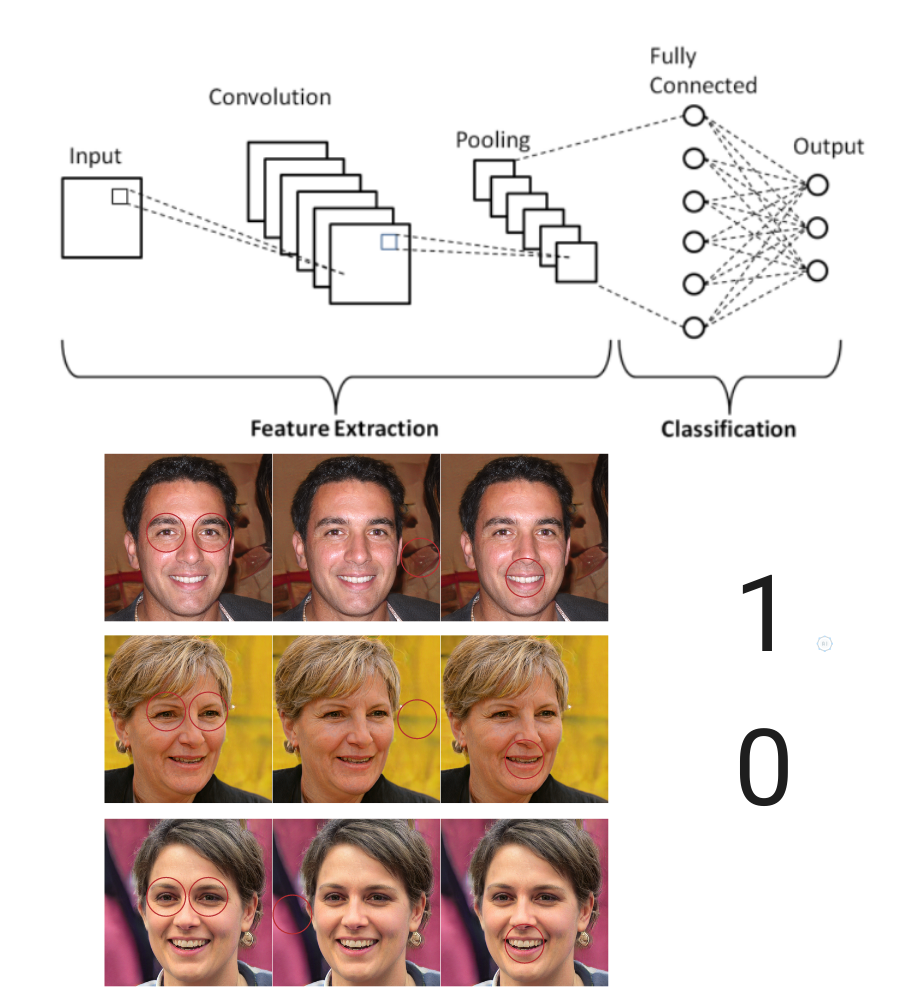
\includegraphics[width=0.5\textwidth]{img/f9.png}}%
\caption{Possible Architecture of CNN applied to the StyleGAN problem \citep{Karras2019, OShea2015}}%
\label{fig:9}%
\end{figure}

The network architecture of a CNN is divided into three dimensions categorised as the convolutional layer, pooling layer and fully-connected layer \citep{OShea2015}. The dimensionality created by the stacked layers sets CNN's apart from ANN's in image classification. The first layer in a CNN distinguishes it from the standard ANN and produces improved performance when it is implemented for image classification.

When the input is passed through this layer, the convolution applies various filters on the data to activate two-dimensional maps \citep{OShea2015}. These 2D maps determine if features are present in the image based on pixels activated when filtered on the activation maps. The convolutions within this network can get large in dimensionality, and the pooling layer is responsible for reducing the complexity of the calculated data \citep{OShea2015}. The function of the pooling layer to reduce the dimensionality of the network can be detrimental to the data because any dimensional reduction in the architecture of the NN further reduces the data dimension simultaneously. Finally, neurons gather the data directly from nodes in the previous layer and, without connecting the preceding layers, conclude the neural network \citep{OShea2015}.

\begin{figure}[H]%
\centering
\fbox{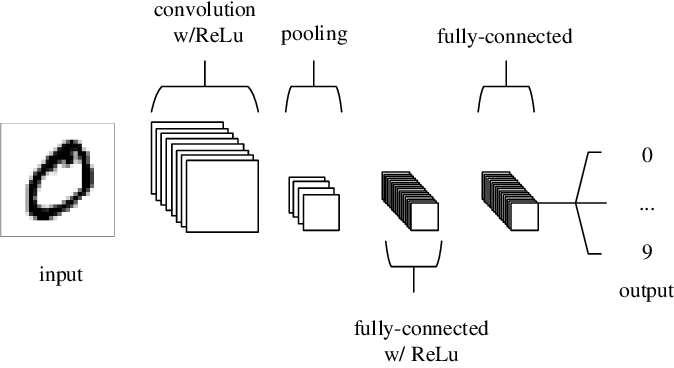
\includegraphics[width=0.8\textwidth]{img/f5.png}}%
\caption{CNN used in the classification of digits \cite{OShea2015}}%
\label{fig:5}%
\end{figure}

Figure \ref{fig:5} visualizes the hidden convolution layer, pooling layer, and the fully connected layers within a CNN. Various iterations of the layers pose different advantages and disadvantages in a practical application.

The benefit when using a CNN on an image processing problem is the improved accuracy in detecting objects within the image \citep{Albawi, Alzubaidi2021}. The activation maps present in a CNN enables the neural network to robustly identify objects within an image through the localisation of the raster data. CNN share weight between its parameter, and this reduces the number of required nodes in training. The reduction in training nodes improves CNN generalisation and reduces overfitting created by the training process. The localisation and object detection of CNN requires extensive calculations, and the process is computationally expensive. This drawback means that without the necessary graphical processing hardware, the training of the CNN will take a long time compared to most other neural networks \citep{Alzubaidi2021}

\subsubsection{Generative Adverserial Networks}

Competition increases the performance of sports athletes, students, and businesses \citep{Burguillo2010,Hays2009,Medvedev2005}. Neural networks can train themselves with the appropriate datasets as identified earlier. With the analogy that a neural network aims to mimic the human brain in its structure, the assumption can be made that competition might increase a neural network's performance. This assumption that competitive neural networks competing against one another led to the formulation of GANs \citep{Creswell2018}.

GAN's use a discriminator and generator to produce two neural networks competing against one another \citep{Creswell2018}. The result of pitting two networks to compete against each other leads to the network being able to improve itself more effectively and further increase application possibilities with these types of networks \citep{Goodfellow2014}. The generator constantly tries to fool the discriminator and the discriminator, in turn, try to identify when its input originated from the generator. 
The generator can be characterised as a criminal trying to falsify identification documents and the discriminator as a customs officer checking a passport. The criminal constantly tries to fool the customs officer. When he succeeds, the officer remembers the fake passport he missed in his identification of fake passports, and the process starts again. The officer learned from his mistake and can in future detect fake passports better. When the criminal fails, the process restarts and similar to the officer the criminal also learns from his mistakes and adapts how he generates fake documents \citep{Goodfellow2014}. The generator constantly creates, and the discriminator constantly describes. This cat and mouse game of fooling and detection in training is how a GAN evolves into the robust networks present in the field of fake images created by neural networks.

\begin{figure}[H]%
\centering
\fbox{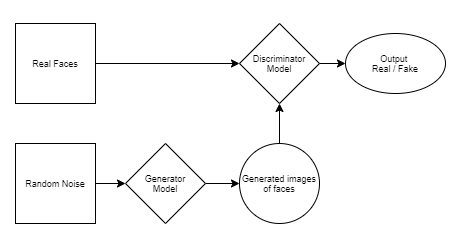
\includegraphics[width=0.8\textwidth]{img/f6.png}}%
\caption{GAN architecture adapted from \cite{Creswell2018}}%
\label{fig:6}%
\end{figure}

A demonstration of how the structure of a GAN allow the discriminator to be critical of the generator output is evident in Figure \ref{fig:6}. The advantage brought on by this neural network architecture is the improved data processing performance. The GAN can process images with sharper resolution than the standard ANN that require images with reduced sharpness for model integrations \citep{Goodfellow2014}. The main disadvantage of implementing GAN is increasing complexity to keep the generator and discriminator synchronised while training the models. 

StyleGAN and StyleGAN2 are GANs with an improved generator that applies specific "styles" on images, and the combination leads to the generation of new images \citep{Karras2019,Karras2020}. A convolutional GAN is a GAN implemented where the generator creates images with convolutional neural network architecture. This combination of the GAN checking against itself while creating images with the architecture of CNN enables improvisation in image generation \citep{Karras2019,Wang}.

\subsection{Activation Functions in Neural Networks}

Activation functions is a crucial part of neural networks and their processing capabilities. Without the presence of activation functions in the nodes of a neural network, the learning of the network will be reduced and the maps between the input and the output will not reach the required complexity. In this literature study an analysis on activation functions, why they are necessary and the different types of activation functions available must be conducted.

\subsubsection{Activation functions are crucial for neural network learning}

Activation functions are the processes on the nodes within the layers of neural networks that allow information to be derived from the data in specific ways. An activation function determines in what way the node will set itself on/off and allow its weight to influence the output of the network. Activation functions are used in an ANN to transform the input signal on a node to the output signal and sequentially add the output of the previous layer to the input of the next layer \cite{sharma2017}.

The inputs and weights are calculated first and then before the output is sent to the next layer the activation function is applied on the node \citep{sharma2017}. Accuracy within neural networks can fluctuate greatly and is influenced by the number of layers within the network and the types of activation functions used. The types of activation functions within the neural network however has a more significant influence on the accuracy of the prediction of the neural network \cite{sharma2017}. There is no clear way to determine the best number of layers a neural network architecture must consist of, but there is a clear consensus between data scientists that a minimum of two layers must be used \cite{sharma2017}.

In neural networks, there are different types of activation functions but the most common set of these functions is the non-linear activation functions \citep{sharma2017}. In neural network activation functions, there are boundaries present and these boundaries describe the type of activation function a specific approach consist of, in a linear activation function this boundary is linear \citep{sharma2017}. Because of these linear boundaries in linear activation functions, the neural network will only be able to change its perception of the data in linear increments. The problem however faced with these activation functions is that real-life scenarios and problems the errors present consist of non-linear characteristics \citep{sharma2017}. Therefore data scientists opt for non-linear activation functions over linear activation functions in their functional neural network implementations.

In the development of the artefact the use of non-linear neural networks will ensure that complex information will be processed from the initial dataset. By adding non-linear activation functions to the neural network the output and steps toward the output will be non-linear in the result. 

The most important aspect of using activation functions is that the functions are differentiable so that backpropagation optimization can be implemented. When backpropagation can be implemented with the use of gradient descent will the neural network have the capability of calculating the errors and losses based on the calculated weights its uses within its layers \citep{sharma2017}.

\subsubsection{Different types of activation functions}

Different types of activation functions can be used and implemented on the layers within the neural network. The type of activation function that can be used depends on the data set and properties present in the data, and the output required from the data. As an example for binary image classification the layers in the network will have to consist of ReLU activation layers, yet the final output layer must be a Sigmoid activation layer.

\begin{table}[H]%
\caption{Different Activation Functions in Neural Networks \citep{sharma2017}}
\label{tabl:actfnn}
\centering
\small
\begin{tabular}{cccccc}
\hline
\\ Linear & Sigmoid & Tanh & ReLU & SoftMax & ExpoLU \\
\hline
\end{tabular}
\end{table}

In the review on activation functions it is apparent that activation functions is a crucial aspect of neural networks and the successful output that neural network can present. Activation functions have a bigger impact on the prediction accuracy of a neural network than the number of layers present within the neural network. There is still some guessing involved into which functions will result in the best accuracy predictions of the neural network but to some degree, there is a clear consensus as to what function will work best with specific types of data. Image classification is improved with the use of ReLU functions throughout the neural network layers and a Sigmoid activation functions as it finals output layer.

With the evaluation of CNN and GAN, an understanding of neural networks in the context of the aim of this project was conducted. CNN provides enhanced capabilities in the generation and classification of image data. While GAN provides specific alterations to images and specialized focus on own output validation and improvement. For the neural network training on a dataset containing authentic images and StyleGAN generated images, supervised learning is the appropriate choice. The architecture and learning paradigms choices for neural networks should be influenced by the type of application and datasets used within training, and because of this, a CNN neural network with semi-supervised learning will be used in the development of the project's artefact.

\section{StyleGAN}

StyleGAN brought new developments in applying styles on images and changing these styles to morph images into new unique style based changes \citep{Karras2019}. Fraudsters are empowered to better create fraudulent identities by applying these styles to images of faces. A fraudster can use StyleGAN to apply styles on their faces to change how they are perceived at checkpoints and more. StyleGAN still introduced advantages to the field; however, the detection of these images is necessary in today's media-centric world. The technology of StyleGAN generated images must first be understood to create a successful implementation technique to detect the generated images.

The StyleGAN addition to the vast sets of different neural networks implemented on different problems originated sequentially with the advances made in the fields of convolutional neural networks and GANs. Because of the computational advances of CNN discussed earlier StyleGAN improved in its generation of new images. StyleGAN2 further improved on this by reducing artefacts brought on in combining styles using the GAN from StyleGAN \citep{Karras2020}.

\subsection{StyleGAN Architecture}

The structure of StyleGAN differentiates it from normal GANs and allows for the combination of "styles" to create new images of non-existing humans \citep{Karras2019}. StyleGAN initializes with an insertion of the base image and input parameter of what styles need to be applied to that image, such as age, sex, and race. Applying all these parameters in the neural network leads to an image being created that changes the styles in the base image. StyleGAN architecture altered the architecture of the generation model to allow for more control over generating with different styles.

Figure \ref{fig:7} illustrates the original StyleGAN network architecture and compares the StyleGAN architecture to the architecture of a traditional GAN. The mapping of the styles added to the architecture of traditional GANs present and a clear indication of how StyleGAN can apply the styles within images can be seen.

\begin{figure}[H]%
\centering
\fbox{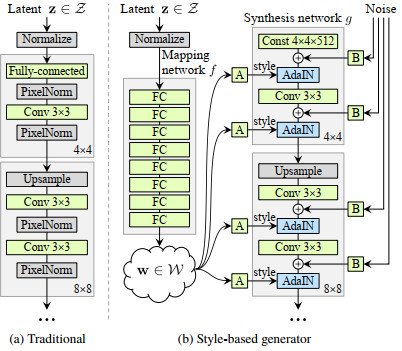
\includegraphics[width=0.6\textwidth]{img/f7.png}}%
\caption{Network architecture of StyleGAN vs Traditional GAN's \citep{Karras2019}}%
\label{fig:7}%
\end{figure}

Differences in authentic images and StyleGAN images are minimal. The most noticeable differences are the artefacts that StyleGAN generates due to deficiencies within the StyleGAN technology. These artefacts vary from rain-drop blotches in images to hair strands not showing realistic definition \citep{Karras2020}. In the second iteration of StyleGAN, the artefacts were addressed with minor improvisations but remain present in StyleGAN2 images \citep{Karras2020}.

Figure \ref{fig:8} illustrates artefacts present in StyleGAN generated images. This water drop effect present in these images could be more accessible for humans to identify than for a neural network due to the generalization of raster data \citep{Karras2020}.

\begin{figure}[H]%
\centering
\fbox{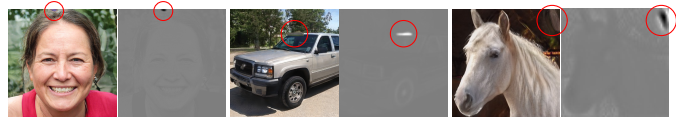
\includegraphics[width=0.95\textwidth]{img/f8.png}}%
\caption{Artefacts present in StyleGAN generated images adapted from \cite{Karras2020}}%
\label{fig:8}%
\end{figure}

\subsection{Detection of CNN Generated Images}

To detect StyleGAN generated images, the discriminator of the initial neural network can, in theory, be isolated and used to detect images created by the generator. The generator recurrently aimed to fool the discriminator, and the discriminator constantly adapted to the generator \citep{Karras2020}. The isolation of the discriminator is an invalid approach to detection because of how learning takes place within the creation of the StyleGAN network and when stoppage occurred in the training phase of the initial technology. The discriminator stops training before the generator, and thus an isolated discriminator will not be able to detect the output of the improved generator. In StyleGAN, the discriminator is not available to the public and to isolate it would require retraining of the GAN with the initial datasets of Flickr Faces images. A basic technique of supervised training to detect CNN generated images was implored by the researchers, and their results proved successful in detecting generated CNN images \citep{Wang}.

\begin{table}[H]%
\caption{Results of \cite{Wang} detecting various CNN's generating images}
\label{tabl:1}
\centering
\small
\begin{tabular}{ccc}
\hline
CNN-image generator & Detection accuracy of \citep{Wang}\\ 
\hline
ProGAN & 98.8\% \\
StyleGAN & 99.6\% \\
BigGAN & 66.4\%\\
CycleGAN & 88.7\%\\
StarGAN & 87.3\%\\
Deepfake & 58.1\%\\
\hline
\end{tabular}
\end{table}

\cite{Wang} proved that by employing a neural network to train labelled images as either real or faked, CNN-generated images could be detected. Table 1 results from their application of different image generation or changing neural networks. The success that \cite{Wang} achieved demonstrated that a semi-supervised neural network can detect CNN-generated images. Therefore a simple neural network approach is validated, and in the context of detecting StyleGAN images, a similar approach will be taken.

The basic architecture and structure of the generator of StyleGAN discussed previously gives more understanding of how StyleGAN can create such precise replication images of human beings. The success of a previous form of detection was evaluated, and StyleGAN images can be detected. By evaluating the work conducted by \cite{Wang}, a primary neural network with semi-supervised training is identified as a solid foundation for further detecting StyleGAN generated images.

\section{Summary}

Through this literature study, research and developments surrounding StyleGAN, neural networks, and different network architectures and learning paradigms were evaluated and discussed. CNN can create or detect images utilizing the strong computational power provided. GAN can change or initially create derived images, and StyleGAN can implement further control over the changes in the generated images. The types of neural networks involving StyleGAN and other surrounding technologies were evaluated, and an approach was discovered. A simple neural network utilizing semi-supervised learning will train on StyleGAN generated images and authentic images of human faces contained in the Flickr faces dataset will it be possible to detect these generated images as initially discovered by \citep{Wang}. The knowledge gained throughout this literature review will be used to develop the artefact to detect StyleGAN images. The development of the final artefact that detects these images will form the third chapter in this project
\chapter{Development of the Artefact}\label{ch3}

The problem of StyleGAN generated faces aiding in the malicious creation of false identities confirmed in the crackdown of Facebook profiles as shown by \cite{Chandler2016} and in the new addition of StyleGAN3 where the creator Nvidea also emphasized the problem and research aiming to detect these images \citep{Karras2021}.

In this projects literature study it was identified that a machine learning deep neural network approach will be the simplest solution to the problem. A neural network that can identify images as either real human images or images generated by StyleGAN with relative accuracy as a method for detection must be implemented in an easy to use front end for the aims of this project to be satisfied. The proposed method of detection should be the easiest solution to the problem as substantiated by \cite{rasmussen2001} with their findings concluding that a simple neural network is usually the best neural network.

\section{Artefact Description}

The artefact for this proposed project can be divided into two main aspects namely the neural network model that will train on 2 separate datasets to classify new images between the characteristics of the data classes it learned in trained. The second aspect is the minimal front-end that will allow users to easily interact with the neural network model and receive simple output on the identification of their uploaded images. The neural network was created using the python programming language in a Jupyter notebook that was compiled and executed on the Google Colab virtual cloud-based environment. To create the neural network popular machine learning packages in the python language was used namely Keras and TensorFlow. The neural network was evaluated and determined to be sufficient, but improvisations could be made using the new technology Optuna for hyperparameter optimization. The neural network was then implemented in a minimalistic front end web app using the python web framework Flask.

\section{Artefact Life Cycle}

The development of the artefact was conducted with the use of DSRM and an Agile combination as stated in  Chapter \ref{ch1}. The DSRM  

\section{Description of the Development of the Artefact}

As stated in the methodologies used in Chapter \ref{ch1} and the Artefact Life Cycle the development of the artefact in this project was subdivided into Sprints. Each sprint handled a subset of tasks to allow for a manageable section of development. This partitioning of the overall workload aided in the development of the artefact and the subsequent testing of the implementations to ultimately ensure a successful project compared to the initial project aims and objectives. Therefore the overall artefact development will be discussed in terms of these sprints. The software used and implemented as well as the final implementation of the method of detection will be structured out in these sprints. 

\section{Sprints}

In the development of the artefact, the overall workload was subdivided into 4 separate sprints. In the 1\textsuperscript{St} Sprint the datasets were retrieved and compiled and an initial neural network was created. The 2\textsuperscript{Nd} Sprint entailed training the neural network and evaluating the accuracy of the model in detecting StyleGAN generated images. The 3\textsuperscript{Rd} Sprint used the results of the evaluation in the 2\textsuperscript{Nd} Sprint and it was determined that improvements could be made. Optuna was used to improve the neural network model. The 4\textsuperscript{Th} and final sprint completed the method of detection by implementing the neural network into a minimalistic front-end web application using the Flask framework.

\subsection{Sprint 1}

In the 1\textsuperscript{St} Sprint of the development of the artefact the StyleGAN dataset was downloaded from the official StyleGAN GitHub repository where various datasets are included of StyleGAN generated images. For the images of real human faces, the FlickrFaces dataset was retrieved from the FlickrFaces GitHub repository. The original datasets contained 100 000 images each and for the detection of StyleGAN images, a subset was created of these datasets that reduced them in size by the number of images and included them together in a dataset that can be used in the training of the neural network model \citep{Karras2019}.

\subsubsection{Downloading and the Dataset}

The datasets that are provided by StyleGAN and the FlickrFaces dataset each contain 100 000 high-quality images. The problem however that was faced is that these high-quality image datasets were also very large. Conventionally datasets used and sometimes contained in software such as Google Colab and Kaggle is small in total size. The StyleGAN high quality generated faces image dataset size was a total of 175GB and the FlickrFaces dataset total size was 140GB. 

The two datasets were made available on their respective GitHub repositories, redirecting to the file buckets hosted in Google Drive. To access the data locally the drives were shared to an NWU institution Google Drive account which does not have a storage limit. In Google Drive shortcuts to the original datasets could be added to the home directory of the account. the datasets could then be downloaded from the home directory.

The problem however faced when using this method is the internet limitations posed on campus at the North-West University's Potchefstroom campus. When downloading through a browser using on-campus internet infrastructure the connection will be throttled if a single file larger than 1GB is downloaded. Google Drive automatically compresses downloads into zip files when downloading and individual files cannot be downloaded sequentially using the internet browsers. Speeds up until 1GB downloaded would stay constant and at high-capacity then after reaching 1GB would be throttled down to low inconsistent speeds. A better way to retrieve the datasets locally had to be used.

\begin{figure}[H]%
\centering
\fbox{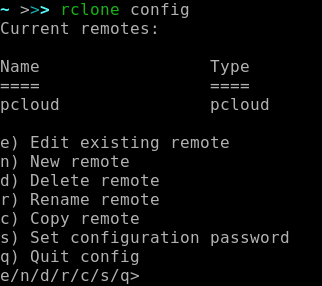
\includegraphics[width=0.5\textwidth]{img/f10rclone.png}}%
\caption{rclone setup config example \citep{rclone2021}}%
\label{fig:10}%
\end{figure}

To address the problem of internet speeds being throttled when downloading the datasets the command-line software rclone was used. rclone, a Linux native package, was installed on the windows local system using the dedicated windows installer. As demonstrated in Figure \ref{fig:10} rclone could be opened up in the command line and after mounting a connection to the Google Drive account could the whole dataset be downloaded sequentially. Each file is downloaded individually from the Google Drive dataset to the local machine, and the total download times of both datasets are completed overnight.

\subsubsection{Dataset Preparation}

The datasets had to be compiled together into one dataset that was used within training the neural network. When training a neural network for a binary image classification problem the dataset directory structure is an important aspect of the data. When the neural network trains and validates its training it compares its prediction with the original image file directory in both training and validation. If the network predicts an image to be StyleGAN generated it checks its prediction against the folder in which the file is located. The subdirectories for the datasets created in this project followed a similar structure to that of the Cat-vs-Dog problem that is used when learning about binary image classifications in neural networks. Table \ref{tabl:folders} shows the structure of the dataset, this directory structure remained the same for all subsequent datasets as they were created to address the resources problems that were identified in Sprint 2 and for the hyperparameter optimization trails in Sprint 3.

\begin{table}[H]%
\caption{Folder Structure of the dataset used in identifying StyleGAN images}
\label{tabl:folders}
\center
\small
\fbox{
  \begin{forest}
    for tree={font=\sffamily, %grow'=0,
    folder indent=.9em, folder icons,
    edge=densely dotted}
    [\textbf{Dataset}
      [train, this folder size=20pt
          [ff]
          [sg]]
      [valid, this folder size=20pt
          [ff]
          [sg]]
      [test, this folder size=20pt
          [ff]
          [sg]]    
      [\textit{vectorize.py}, is file]
    ]
  \end{forest}
  }
\end{table}

Initially, the subset created from the StyleGAN and FlickrFaces datasets retrieved consisted of 20 000 images. The number of images used for the identification of StyleGAN images was decided based on the findings of \cite{Nasr2016}, that concluded the more images a neural network can use in image classification the better its prediction will be. To an extent, this is true for the problem of StyleGAN generated images versus images of real human faces due to the fine differences between the two types of images. The neural network won't classify the images based on the shape as in the Cat-vs-Dog problem but will rather focus on the small artefacts or features that are present in StyleGAN images for its classification. 

Using too large a dataset can lead to the neural network overfitting the data \citep{Trask2019}. Overfitting occurs when the created neural network model becomes exceptionally good at being classifying the dataset it trained on, but performs much worse when classifying data that it was not trained on. Because of the scope of the proposed project the neural network that is created does not have to be the "\textit{perfect}" model, and will in a sense overfit facial recognition features as that is the premise for the creation of the model. What this means is that if the model created gets an input image of a car and classifies it as a real human or a StyleGAN generated image, this form of overfitting is acceptable in the context of the scope of this project. Figure \ref{fig:11} illustrates the acceptable amount of overfitting that can be expected from the neural network. The network however must not overfit the images included in the training set of real human faces retrieved from the FlickrFaces dataset, as then it will classify all images as StyleGAN if it was not in the FlickrFaces training set. This issue is addressed in the second sprint when the initial neural network is created. 
  
\begin{figure}[H]%
\centering
\fbox{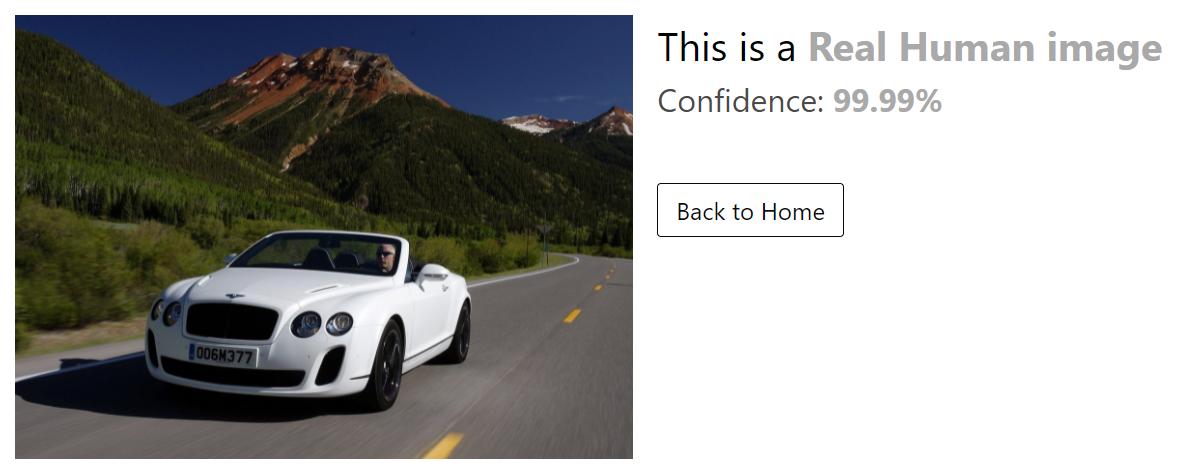
\includegraphics[width=0.7\textwidth]{img/f11.png}}%
\caption{Acceptable level of Overfitting for the StyleGAN identification model}%
\label{fig:11}%
\end{figure}
  
A subset of these 2 datasets will improve the development of the artefact as working with a large dataset while testing and implementing hot and cold learning will unnecessarily increase the development time. Training times are influenced by the number of epoch in training and the number of samples used. When developing a neural network works it is standard to use a small subset of the training set to keep the times in testing lower, and after the development of the neural network is completed move over to the full dataset. The Full dataset that will be used in the final training and optimization of the neural network will be larger than the small dataset used in development to ensure that the final model can identify the features present in StyleGAN generated images. Table \ref{tab:sizes} states the sizes of the datasets and the subdirectories that will be used in the development and the final optimization of the neural network model. 

\begin{table}[H]
\caption{Total amount of images used in the Artefact creation}
\label{tab:sizes}
\resizebox{\textwidth}{!}{%
\begin{tabular}{lllllll}
\hline
Directory & \multicolumn{2}{c}{Development} & \multicolumn{2}{c}{Training} & \multicolumn{2}{c}{Optimization} \\ \hline
\multicolumn{1}{|l|}{} & \multicolumn{1}{c|}{sg} & \multicolumn{1}{c|}{ff} & \multicolumn{1}{c|}{sg} & \multicolumn{1}{c|}{ff} & \multicolumn{1}{c|}{sg} & \multicolumn{1}{c|}{ff} \\ \hline
\multicolumn{1}{|l|}{Train} & \multicolumn{1}{l|}{1000} & \multicolumn{1}{l|}{1000} & \multicolumn{1}{l|}{2000} & \multicolumn{1}{l|}{2000} & \multicolumn{1}{l|}{4000} & \multicolumn{1}{l|}{4000} \\ \hline
\multicolumn{1}{|l|}{Validation} & \multicolumn{1}{l|}{500} & \multicolumn{1}{l|}{500} & \multicolumn{1}{l|}{1000} & \multicolumn{1}{l|}{1000} & \multicolumn{1}{l|}{2000} & \multicolumn{1}{l|}{2000} \\ \hline
\multicolumn{1}{|l|}{Test} & \multicolumn{1}{l|}{500} & \multicolumn{1}{l|}{500} & \multicolumn{1}{l|}{1000} & \multicolumn{1}{l|}{1000} & \multicolumn{1}{l|}{2000} & \multicolumn{1}{l|}{2000} \\ \hline
Total Dataset Size &  & 4000 &  & 8000 &  & 16000 \\ \hline
\end{tabular}%
}
\end{table}

Table \ref{tab:sizes} and Table \ref{tabl:folders} shows the layout of the directories that must be consistent throughout the training of the neural network model in the artefact creation. In binary image classification, the process of training a neural network to classify two sets of images into two separate classes, the neural network references the directory in which an image resides for its check on its prediction. This means that in the training stages the neural network will make its prediction on an image, and check if that image is in the real human directory (ff) or the StyleGAN generated images directory (sg) and then change its weights according to the correlation between its prediction and the directory path of the image receives. In short, the neural network will use the directories to "\textit{know}" what type of image the received training image is. 

The validation folder in the directory is the set of images the neural network uses to check its accuracy after each training step while training its weights. The neural network changes its weights after each image in the training set and just uses the validation set as a benchmark for each checkpoint in training. The Test set is important as it will be used to evaluate the final model. The Test set must be kept aside and never accessed in the training phase of the model. Thus a Test set was created early with unique images the will not be accessed again in the training phases.

\subsubsection{Creating the First Neural Network}

For the creation of the Artefact, it was identified that the problem of identifying StyleGAN generated images required binary image classification. To understand how binary image classification could be applied to a StyleGAN problem the Cat-vs-Dog example was used to understand binary image classification. The Cat-vs-Dog problem can be seen as a Hello World exercise that will teach the base fundamentals of binary image classification and the knowledge gained in this problem will be applied to the StyleGAN problem \citep{cat2014}. The Cat-vs-Dog problem is a basic exercise to create a neural network to classify images as either a cat or a dog, and the dataset used in this exercise contains 4000 images of both cats and dogs with image sizes of 200px by 200px. 

The StyleGAN problem was applied to this exercise by using the StyleGAN dataset instead of Cat-and-Dog images. A problem was identified with this implementation as StyleGAN images are very large compared to other datasets used in CNN neural network implementations, namely the MINST handwriting dataset and the Cat-vs-Dog dataset. StyleGAN images and FlickrFaces images native resolution is 1024px by 1024px, which could not be passed to a neural network catered for the classification of Cat-vs-Dog images as the input layer of the neural network must match the image resolution in CNN's \citep{cat2014, Wang}. Figure \ref{fig:13} shows the input layers and image sizes in identifying StyleGAN images and the Cat-vs-Dog exercise.

\begin{figure}[H]%
\centering
\fbox{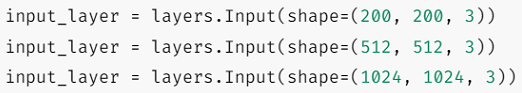
\includegraphics[width=0.95\textwidth]{img/f13.png}}%
\caption{Input layer of the neural network according to the image sizes}%
\label{fig:13}%
\end{figure}

In Figure \ref{fig:12} a comparison between a dog image retrieved from the Cat-vs-Dog dataset and the dataset used for the identification of StyleGAN images in this project with the sizes of the original images (1024x1024px) the scaled-down (200x200px) images to fit into the input layer of the Cat-vs-Dog problem. 

\begin{figure}[H]%
\centering
\fbox{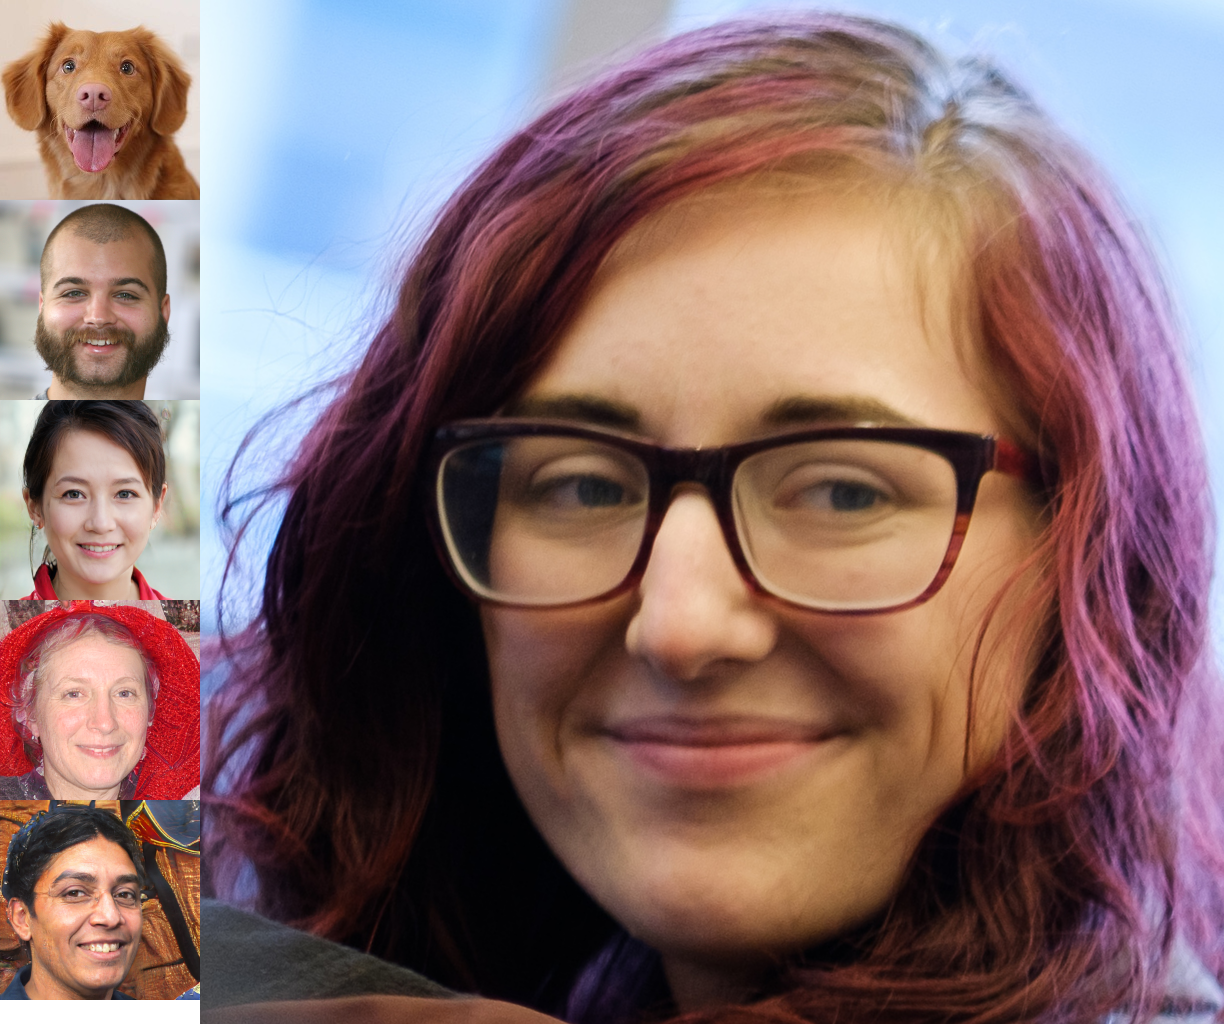
\includegraphics[width=0.9\textwidth]{img/f12.png}}%
\caption{Image sizes of Cat-vs-Dog dataset, rescaled artefact dataset and StyleGAN original sizes}%
\label{fig:12}%
\end{figure}

When the StyleGAN images were passed into the Cat-vs-Dog neural network with a change in the input layer of the network to accommodate full resolution StyleGAN images a usage limit was reached on Google Colab. This identified that some image processing will be required on the dataset. When the images were scaled down to 200x200px and the Cat-vs-Dog neural network trained on StyleGAN images an accuracy of 61\% was achieved. The accuracy achieved with this basic implementation was used as a proof of concept and showed that it was possible to identify StyleGAN images with a neural network. The accuracy of the network however was not ideal and thus a network specific to the StyleGAN problem had to be created.

\subsubsection{Image Processing}

As mentioned in the previous section, the dataset of images gathered for the identification of StyleGAN images had to be processed to allow the neural network to train on these images. Image processing is an entire field on its own with theory relating to it. For the image processing needs to be required in this stage of the artefact development the python library OpenCV was identified to be the simplest solution to the problem being faced. 

OpenCV is a programming library geared mostly at real-time computer vision. It was created by Intel and then supported by Willow Garage and Itseez. Under the open-source Apache 2 License, the library is cross-platform and free to use \citep{opencv2012}. A python script was created to change the entire dataset sequentially and the need to manually scale the image was avoided. The script was used to create different datasets for later use in this proposed project. The image resolutions of the different datasets created included a 200x200 pixels, 512x512px and 1024x1024px.

%too many trainable parameters
%take too long exhaust resources
%the more data the better but nn can work with little

\subsubsection{Summary}

The first sprint in the development of the artefact required the dataset to be retrieved, structured and the images processed. The dataset was downloaded using the rclone program to avoid the throttling limitation experienced. The layout of the directories in the dataset that was compiled for the identification of StyleGAN images was structured to enable the dataset to be used in training. The Cat-vs-Dog exercise proved that a StyleGAN identification neural network model could be created and showed that images had to be processed for a neural network to be trained on the limited resources available. For the processing of the images, a python script was created using the open-source image processing library OpenCV.

\subsection{Sprint 2}
 
In the second sprint of the artefact development, the first neural network was created based on the findings in the first sprint and using that dataset gathered and processed in the first sprint. The initial neural network that was created in this phase of the artefact development just required hot and cold learning and was not optimized in any form. Hot and Cold learning as analysed in Chapter \ref{ch1} is an uninformed guessing game in hyperparameter optimization.

\subsubsection{Creating the First Neural Network}

To create the neural network the TensorFlow package was used. TensorFlow is a machine learning and artificial intelligence software library that is free and open-source. It may be used for a variety of applications, but it focuses on deep neural network training and inference \citep{tensor2016}. TensorFlow was used within the Jupyter Notebooks in Google Colab and locally, and was run in the python environment.

 Keras is an open-source software library for artificial neural networks that include a Python interface \citep{kerascnn2017}. Keras serves as a user interface for TensorFlow. Keras supports the TensorFlow package and is used for creating the neural network in the development of the artefact \citep{kerascnn2017}.
 
The initial neural network was then created using TensorFlow and Keras in Google Colab. The Code for the notebooks used can be found in Appendix \ref{AppendixC} and \ref{AppendixD}. As seen in Figure \ref{fig:nn1} the neural network consisted of 3 convolutional layers, a single dense layer and had a total amount of trainable parameters exceeding 17 million. The large amounts of trainable parameters would result in the resources available in Google Colab being exhausted in training. A hot and cold learning approach was taken and with the smaller test dataset, the model was trained and changed until some improvements could be seen. The trained accuracy of this neural network was 51\% at this stage but could be improved more. 

\begin{figure}[H]%
\centering
\fbox{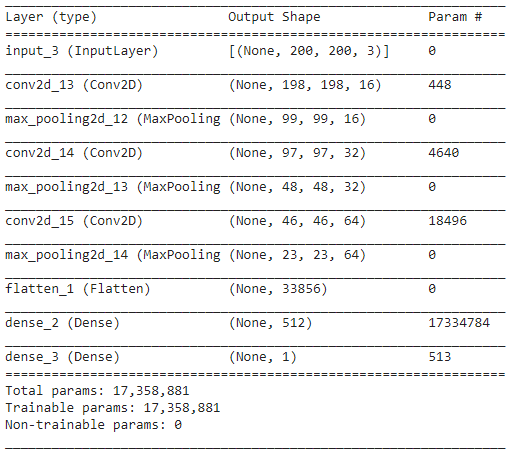
\includegraphics[width=0.65\textwidth]{img/fnnarch1.png}}%
\caption{Summary of Cat-vs-Dog network applied to the StyleGAN problem}%
\label{fig:nn1}%
\end{figure}

More layers and dropout layers were added to the different convolutions using hot and cold learning. Figure \ref{fig:nn2} is a summary of the neural network architecture of a model created for the identification of StyleGAN images using the principles of hot and cold learning applied on the hyperparameters of the model.  

\begin{figure}[H]%
\centering
\fbox{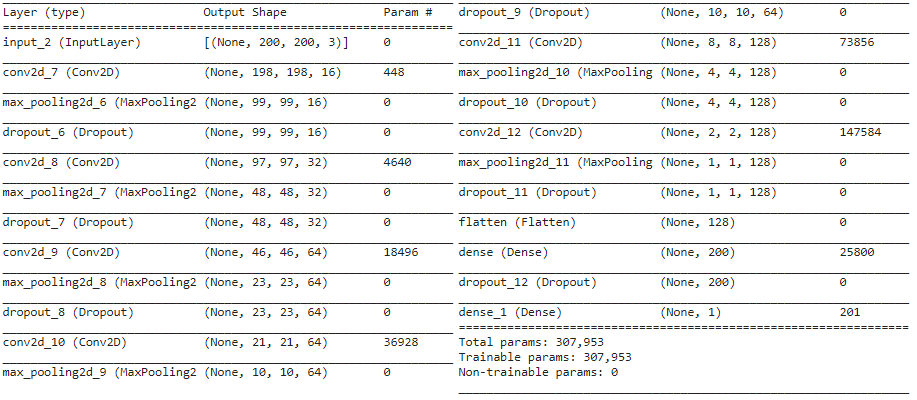
\includegraphics[width=0.95\textwidth]{img/nn2.png}}%
\caption{Summary of the created Neural Network}%
\label{fig:nn2}%
\end{figure}

The final self-created neural network trained on the training dataset could identify the StyleGAN generated images with 81\% accuracy using the test data. The relatively high true accuracy showed promising results but because of the randomness in hot and cold learning and what was identified in the literature review of Chapter \ref{ch2}, the hyperparameters had to be optimized.


\subsection{Sprint 3}

Hot and Cold learning is a viable option for setting neural network parameters when developing neural networks and learning how they can be used to solve problems \citep{Trask2019}. But for the identification of StyleGAN images hot and cold learning proved to be an inefficient manner in which to create the neural network architecture. Optuna was defined as a possible technology to omit the hot and cold learning process and create a highly optimized neural network.  

\subsubsection{Optuna: A hyperparameter optimization framework}

Optuna is a software framework for automated hyperparameter optimization that is specifically developed for machine learning. It has an imperative, define-by-run user interface. The code built with Optuna has a high level of flexibility thanks to its define-by-run Interface, and the user of Optuna may dynamically design the search spaces for the hyperparameters. The phrases "study" and "trial" are used as follows: A Trial is a single execution of the objective function, whereas a Study is optimization based on an objective function \citep{optuna2019}.

When the Optuna hyperparameter process was started in this sprint the trail function and study functions were created based on the documentation of the Optuna framework. The trail is a single iteration in the larger study and the study is a collection of trails where different combinations of hyperparameters are used to reach the goal of the trail. The study goal for identifying StyleGAN images was to increase the accuracy and \cite{optuna2019} terms it was to move the accuracy metric in a maximum position. The trail function was set to suggest a neural network layer count ranging from a single layer network to a 7 layer network. The optimizer was suggested from a pool of optimizers that perform well with image classification problems as was identified by \cite{bera2020analysis} and \cite{kandel2020comparative}. The Study could be changed to also train full neural networks on each trail but it was decided to train the networks the minimal amount just to evaluate the improvements of the models. When the study was completed the resulting model was then trained on the full dataset.

When the Optuna study was executed on Google Colab a problem was faced regarding available resources. Google Colab provides a free service but can throttle users resources based on the amount of resources used. The policies that Google use to dictate what will amount to throttling is unclear and Google can throttle any account based on their discretion. When the Optuna study started the account used on Google Colab for the development of the artefact was throttled down and exceeded the acceptable usage dictated by Google. To work around the problem the jupyter notebooks was downloaded and run on a physical computer provided by Prof. Tiny du Toit. The computer used for the study included a GPU, namely a GTX 1080 with 8GB dedicated graphics memory.

\textbf{Graphics cards differences: compare collab and Nvidia gpu}

\textbf{Image of Optuna output in Study}

\textbf{Train}

\textbf{Image of training}

The model created using the Optuna framework for hyperparameter optimization was trained on the full dataset on the local machine as previously stated and training times were increased due to the improved machine learning factor of the improved GPU. The trained hyperparameter optimized model could identify StyleGAN generated images with an accuracy of 97.3\% and true accuracy of 97.6\% as tested with the python script. The results of the Optuna network compared to the network created in Sprint 1 will be further discussed in the Results chapter in this document.


\subsection{Sprint 4}

With the neural network model completed and trained to exceptional accuracy, a front-end application was created to allow users to easily and intuitively interact with the model as stipulated as one of the objectives of this project. By allowing users to interact with the model easily the aim of identifying StyleGAN images can be satisfied as users will be able to pass images to the neural network that in turn will be able to identify if these images were generated by StyleGAN or if the images are that of real human beings. 

For the front end of the artefact a web application, that will allow for easier deployment and wider reach had to be created to satisfy the objectives of this proposed project. In the final sprint of the artefact development, various frameworks were considered and while developing the artefact it was realised that a python-based web framework will enable the implementation of the neural network. 

\subsubsection{Adding the model to the Web App}

Because the neural network model was created using the Python libraries for machine learning it was realised that a python-based framework will allow the neural network to be implemented in the web app. If another front end framework like React or Angular was used the implementation of the neural network would be unnecessarily complex. React and Angular are JavaScript based frameworks and for the Python model to communicate with the front end of a JavaScript framework an API had to be implemented. The neural network requires the python machine learning libraries TensorFlow and Keras to pass an image through the model and provide the identification as feedback. Thus the libraries must reside in a python environment where TensorFlow and Keras are installed. 

To avoid this added complexity an analysis into python web-based frameworks where conducted and the Django framework stood out. The Django framework however is a very large and clunky framework when compared to the implementation required for the artefact. The child framework Flask, which was derived from Django but with a lightweight footprint was used for the creation of the front-end of the artefact. The Flask app was developed as a minimalistic interface that would guide users intuitively on how to use the app with clear instructions and a simplified design. 

python requires backend

we use TensorFlow and Keras

Django

flask better

artefact looks

home page

UI UX error and 404 

Identified StyleGAN

Identified FF



\section{Summary}
\chapter{Results}
\chapter{Reflection}

\bibliography{MyBib.bib}

\appendix			
\chapter{Ethics Form}

\label{AppendixA}
\begin{minipage}{\textwidth}
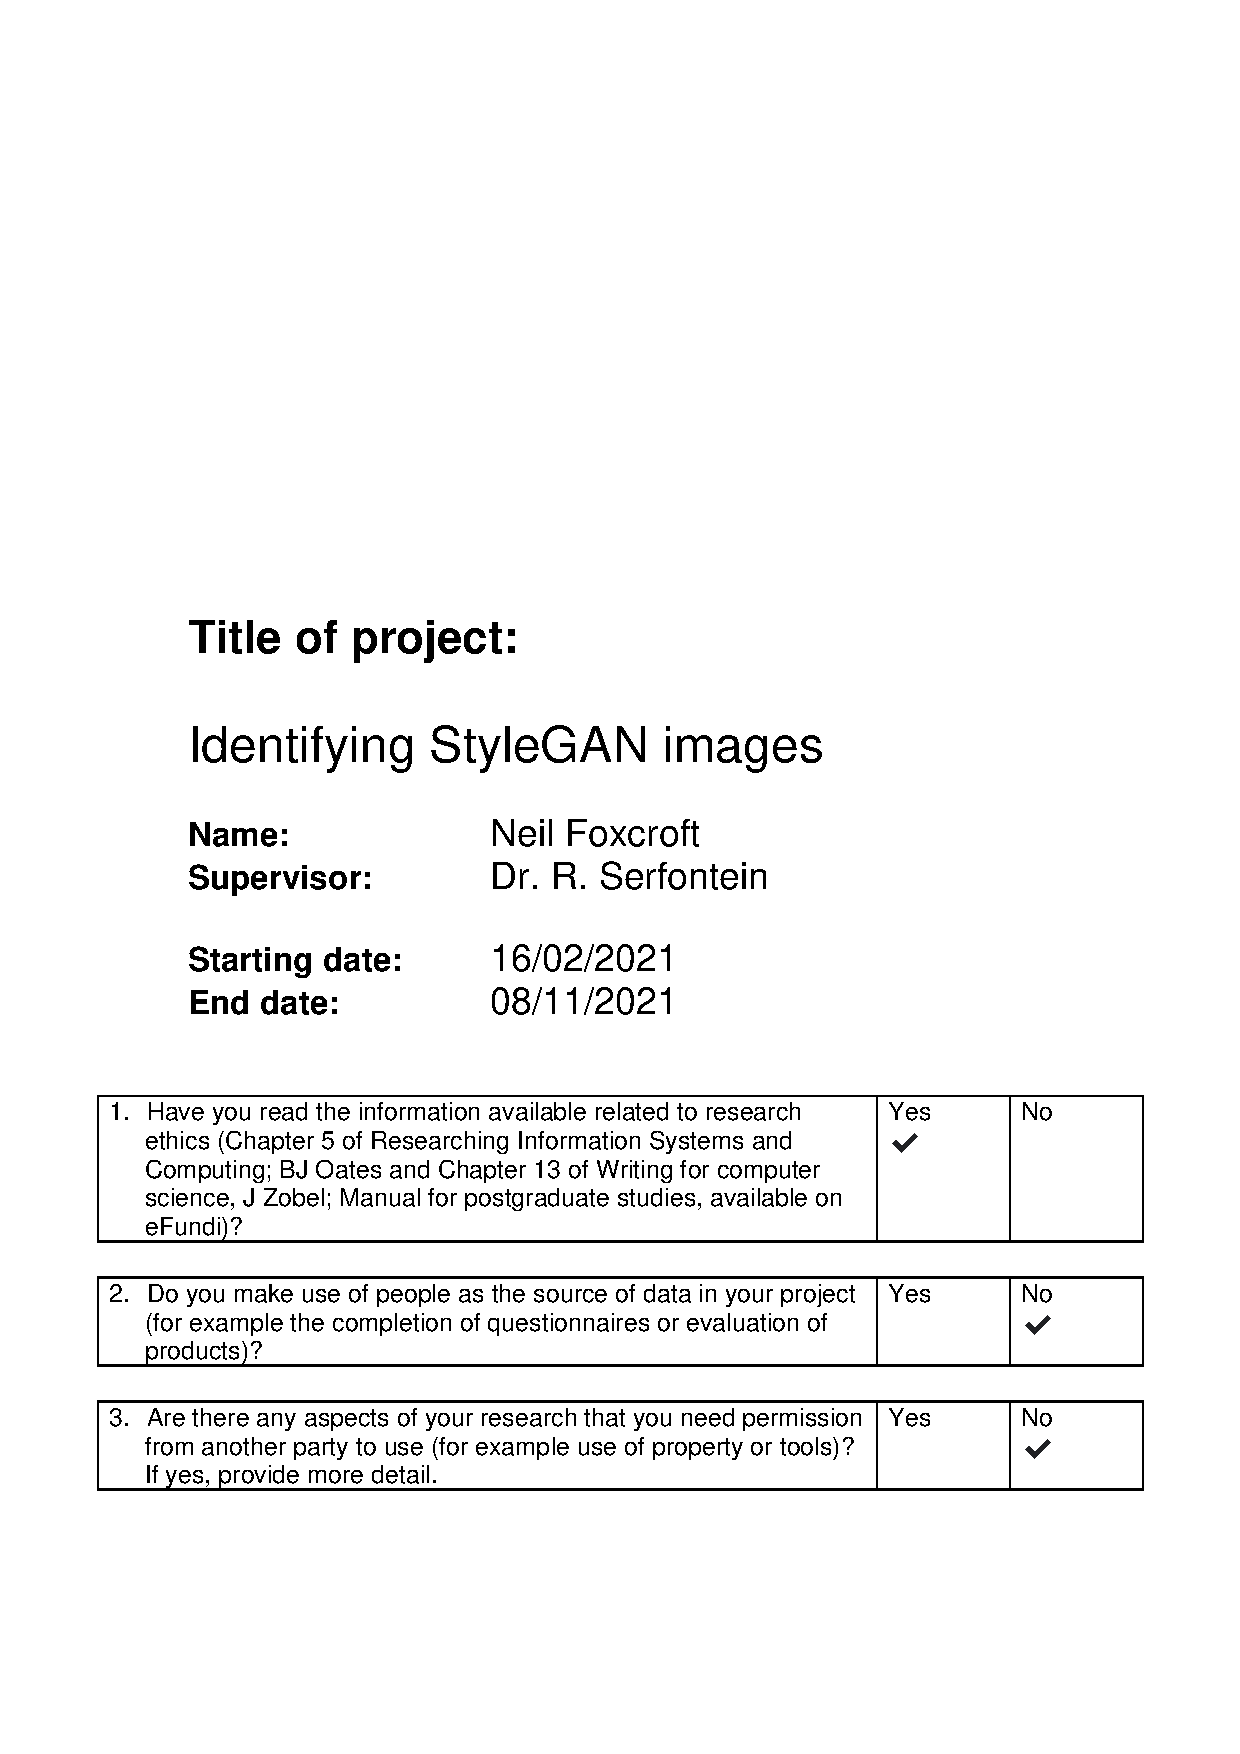
\includepdf[pages=1,pagecommand={}]{forms/ethicsPDF.pdf}
\end{minipage}
\includepdf[pages=2- ,pagecommand={}]{forms/ethicsPDF.pdf}

\chapter{Research Proposal}

\label{AppendixB}
\begin{minipage}{\textwidth}
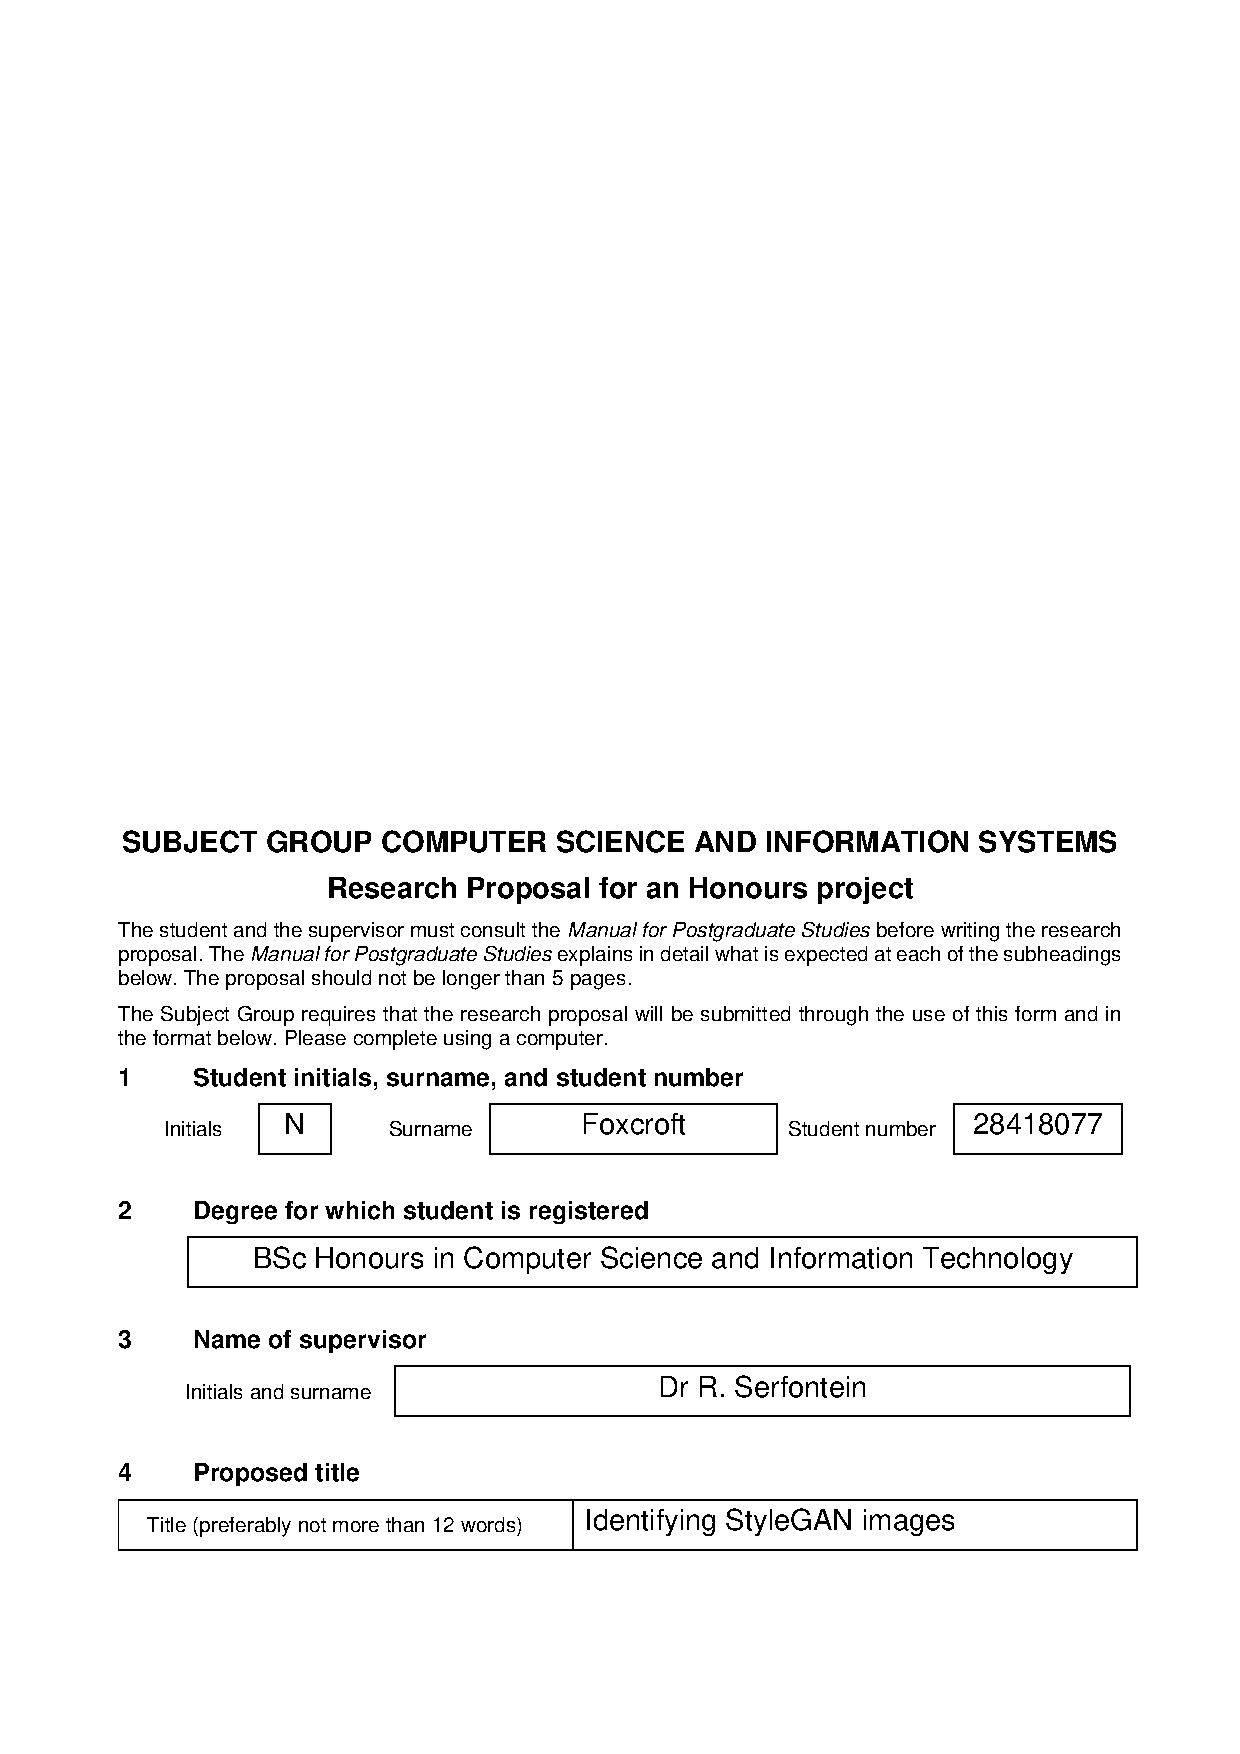
\includepdf[pages=1,pagecommand={}]{forms/proposalPDF.pdf}
\end{minipage}
\includepdf[pages=2- ,pagecommand={}]{forms/proposalPDF.pdf}

\chapter{Jupyter Notebook: 1}

\label{AppendixC}
\begin{minipage}{\textwidth}
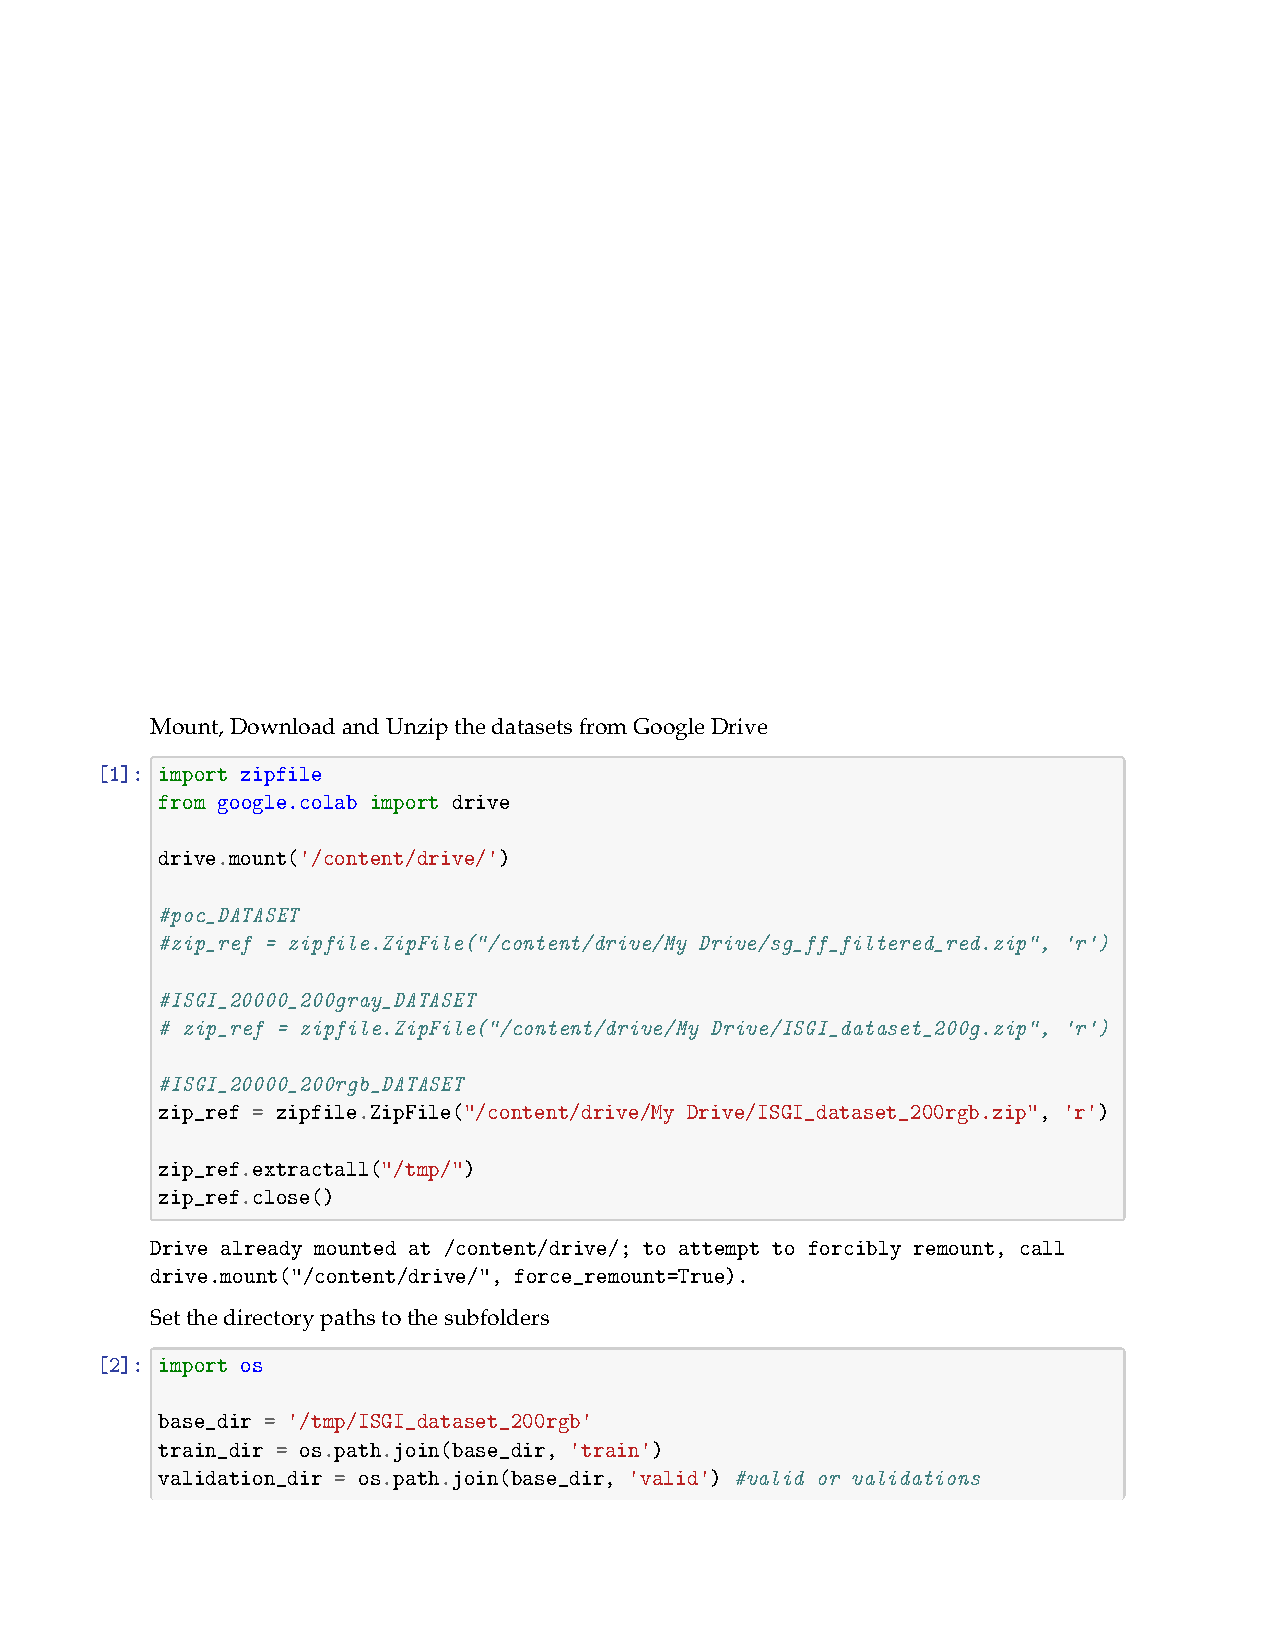
\includepdf[pages=1,pagecommand={}]{appendix/StyleGAN_GS.pdf}
\end{minipage}
\includepdf[pages=2- ,pagecommand={}]{appendix/StyleGAN_GS.pdf}

\chapter{Jupyter Notebook: 2}

\label{AppendixD}
\begin{minipage}{\textwidth}
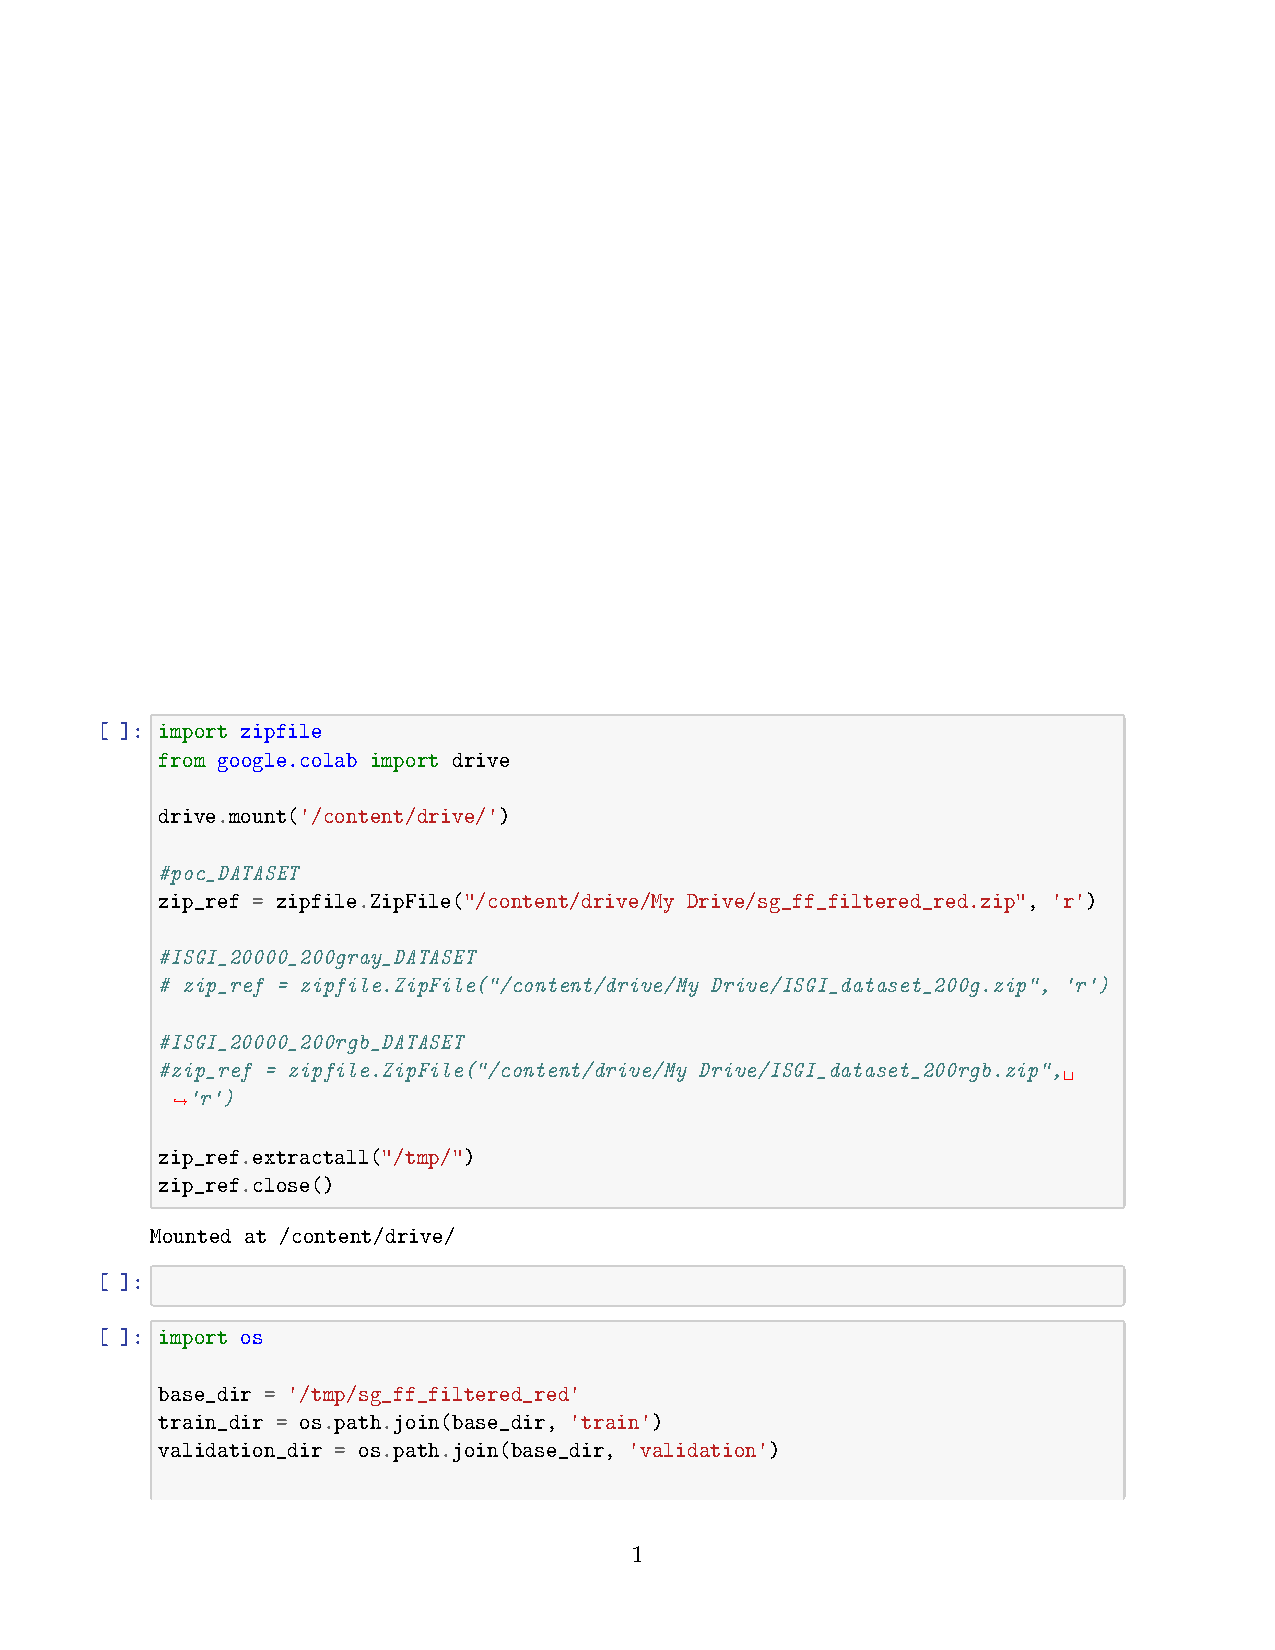
\includepdf[pages=1,pagecommand={}]{appendix/StyleGAN_Optuna.pdf}
\end{minipage}
\includepdf[pages=2- ,pagecommand={}]{appendix/StyleGAN_Optuna.pdf}

\end{document}

